\documentclass[10pt, aspectratio=169]{beamer} %
\usetheme{Singapore}

\usepackage{bookmark}
\usepackage{graphicx}
\usepackage[english]{babel}
\usepackage[utf8]{inputenc}
\usepackage[T1]{fontenc}
\usepackage{amsmath}
\usepackage{color}
\usepackage{listings}
\usepackage{tabularx}
\usepackage{amssymb}
\usepackage{lmodern}

\usepackage{hyperref}
\hypersetup{colorlinks=true, urlcolor=blue}

\DeclareMathOperator*{\minimize}{minimize} %in preamble
 
\newcommand{\N}{{\mathbb{N}}}
\newcommand{\I}{{\bf I}}
\newcommand{\C}{{\bf C}}
\newcommand{\A}{{\bf A}}
\newcommand{\T}{{\bf T}}
\newcommand{\g}{{\bf g}}
\newcommand{\e}{{\bf e}}
\newcommand{\ab}{{\bf a}}
\newcommand{\ba}{{\bf b}}
\newcommand{\Z}{{\mathbb{Z}}}
\newcommand{\R}{{\mathbb{R}}}
\newcommand{\mbf}{\mathbf}
\newcommand{\bs}{\boldsymbol}
\newcommand{\cc}{{\bf c}}
\newcommand{\su}{{\sum_{n=0}^{N-1}}}

\newcommand{\argmax}{\mathop{\text{arg\;max}}}
\newcommand{\argmin}{\mathop{\text{arg\;min}}}

\newcommand{\HH}{{\bf H}}
\newcommand{\thb}{\boldsymbol{\theta}}
\newcommand{\w}{{\bf w}}
\newcommand{\Sigb}{\boldsymbol{\Sigma}}
\newcommand{\mub}{\boldsymbol{\mu}}
\newcommand{\alb}{\boldsymbol{\alpha}}

\newcommand{\s}{{\bf s}}
\newcommand{\SB}{{\bf S}}

\definecolor{blue}{RGB}{32,32,255}
\graphicspath{{./images/}}

\newcommand{\h}{{\bf h}}
\newcommand{\rr}{{\bf r}}
\newcommand{\X}{{\bf X}}
\newcommand{\x}{{\bf x}}
\newcommand{\y}{{\bf y}}
\newcommand{\p}{{\bf p}}
\newcommand{\E}{{\bf E}}
\newcommand{\U}{{\bf U}}
\newcommand{\V}{{\bf V}}
\newcommand{\f}{{\bf f}}
\newcommand{\var}{{\mathop{\text{var}}}}

\newcommand{\F}{{\cal F}}
\newcommand{\leveys}{0.75\textwidth}
\newcommand{\etaisyys}{0.25\textwidth}

\newcommand{\sinc}{\mathop{\text{sinc}}}
\newcommand{\esim}{\em}

\newcommand{\modulo}{\operatorname{mod}}

\setbeamertemplate{frametitle continuation}[from second] 

\renewcommand{\insertcontinuationtext}{}

\setbeamertemplate{frametitle}
{
	\vspace*{0.7cm} \vbox{\insertframetitle}
}

\usecolortheme{default}

\setbeamertemplate{mini frames}{}
\renewcommand*{\slideentry}[6]{}
\setbeamertemplate{frametitle}{
    \vspace*{0.2cm}
    \insertframetitle
}

\title{Pattern Recognition and Machine Learning}
\subtitle{Slide Set 7: Error Assessment and Regularization}
\author{Heikki Huttunen\\
heikki.huttunen@tut.fi}
\institute{Department of Signal Processing\\Tampere University of Technology}
\date{February 2017}

\begin{document}

\maketitle

\lstdefinestyle{mystyle}{
  belowcaptionskip=1\baselineskip,
  breaklines=true,
  frame=single,
  xleftmargin=\parindent,
  language=Python,
  showstringspaces=false,
  basicstyle=\tiny\ttfamily,
  keywordstyle=\bfseries\color{green!40!black},
  commentstyle=\itshape\color{purple!40!black},
  identifierstyle=\color{blue},
  stringstyle=\color{orange},
  moredelim=**[is][\color{red}]{@}{@},
}

\lstset{language=Python,style=mystyle} 


\begin{frame}{Generalization}
\begin{itemize}
\item The important thing is how well the classifier
works with unseen data.
\item An overfitted classifier memorizes the training data and does
not generalize.
\end{itemize}
\centerline{\qquad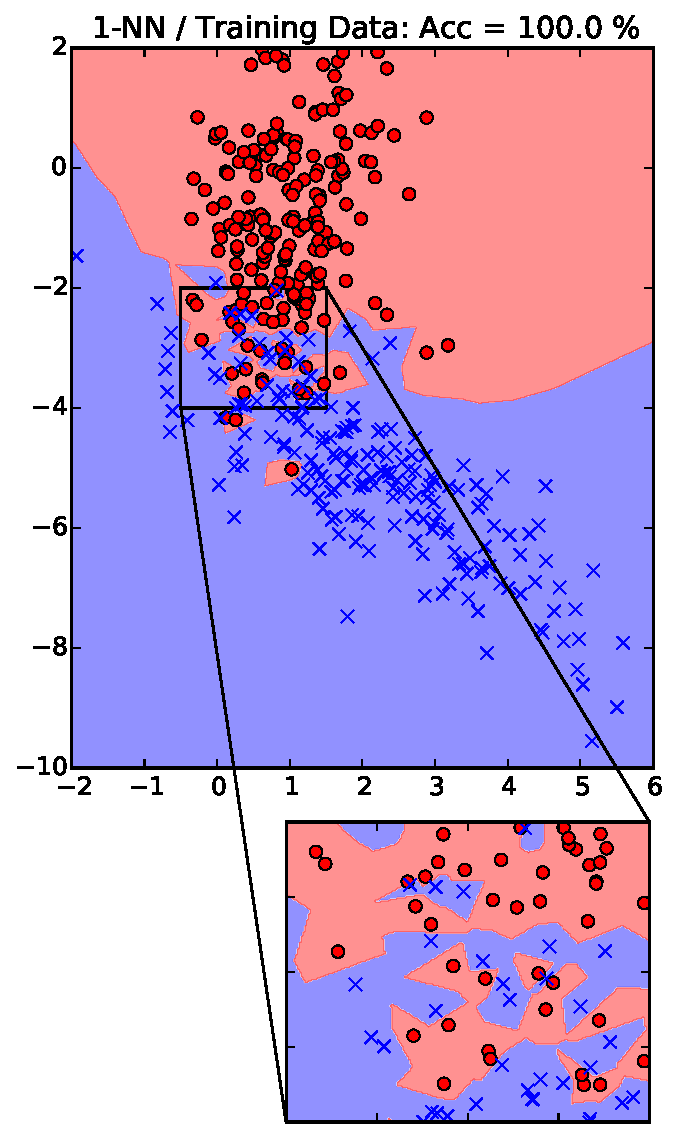
\includegraphics[width=0.25\columnwidth]{1NN-TRAIN.pdf}
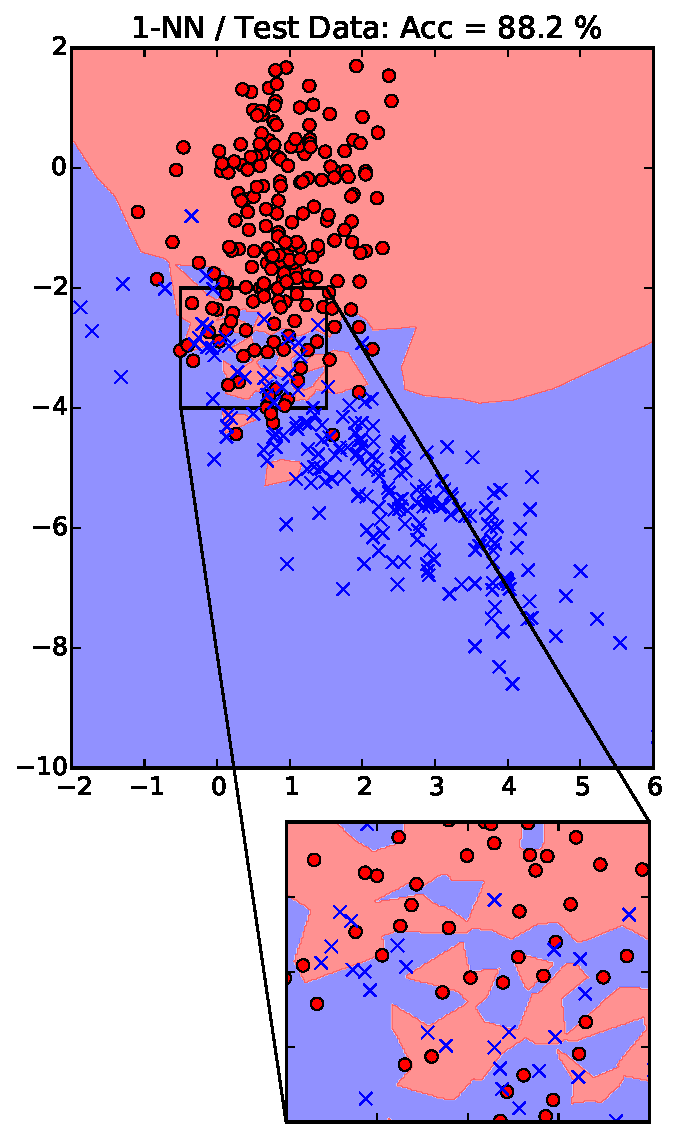
\includegraphics[width=0.25\columnwidth]{1NN-TEST.pdf}}
\end{frame}


\begin{frame}[fragile]{Cross-validation}
\begin{columns}
\column{0.65\textwidth}
\begin{itemize}
\item The generalization ability of a classifier needs to be tested with
\textbf{unseen} samples.
\item In practice this can be done by splitting the data into separate training 
and test sets.
\item A standard approach is to use $K$-fold cross-validation:
\begin{itemize}
\item Split the training data to $K$ parts (called folds)
\item Use each fold for testing exactly once and train with the other folds
\item The error estimate is the mean of the $K$ estimates
\end{itemize}
\item A common value for $K$ is 5 or 10.
\end{itemize}
\column{0.35\textwidth}
\centerline{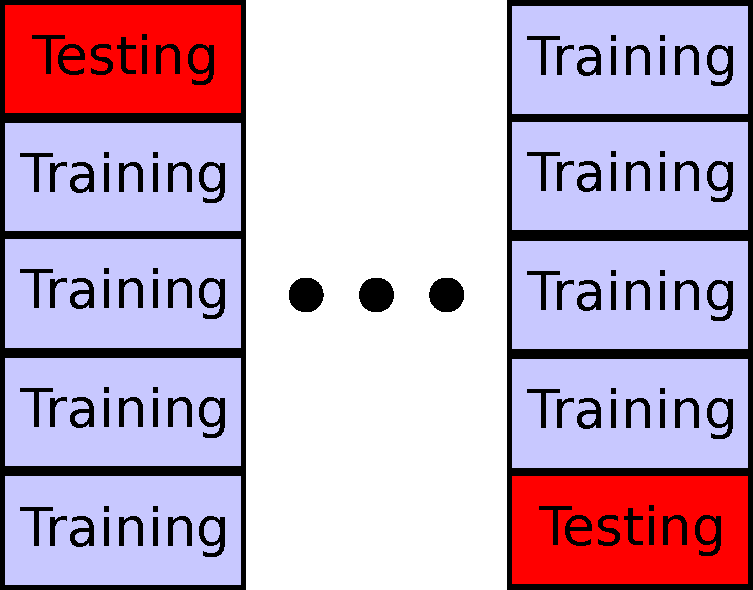
\includegraphics[width=0.8\columnwidth]{CV-Split.pdf}}
\end{columns}
\end{frame}

\begin{frame}[fragile]{Cross-validation in \texttt{sklearn}}
\begin{columns}
\column{0.75\textwidth}
{\small\vspace*{-0.8cm}
\begin{itemize}
\item Cross-validation is extremely elegant in sklearn.
\item Essentially 1 line of code is required:
\begin{verbatim}
from sklearn.model_selection import cross_val_score
scores = cross_val_score(clf, X, y)
\end{verbatim}
\item The cross-validator receives the classifier and the data and
returns a list of scores for each test fold.
\item The function can receive additional parameters that modify the 
number of folds, possible stratification (balancing the classes in folds), etc.
\end{itemize}
}
\column{0.25\textwidth}
{\scriptsize Code:}\\
\fbox{\centerline{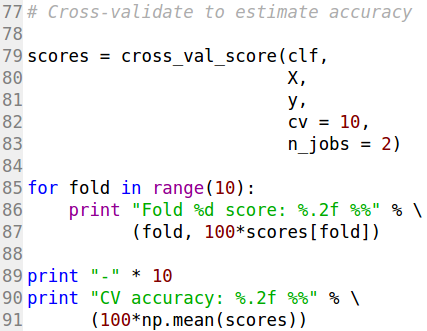
\includegraphics[width=1.0\columnwidth]{cv_code.png}}}
{\scriptsize Result:}\\
\fbox{\centerline{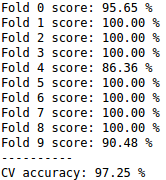
\includegraphics[width=0.6\columnwidth]{cv_result.png}}}
\end{columns}
\end{frame}

\begin{frame}[fragile]{Stratified Cross-validation}
\begin{columns}
\column{0.65\textwidth}
{\small\vspace*{-0.8cm}
\begin{itemize}
\item The CV split can be controlled using the \verb+cv+ argument.
\item Instead of a completely random split, a \textbf{stratified} split is preferred:
Each fold will hold a mixture of classes in same proportion as in full dataset.
\item The stratified split can be generated easily:
\begin{lstlisting}
>>> from sklearn.model_selection import StratifiedKFold
# Generate SKF split. This needs the class labels y.
>>> skf = StratifiedKFold(y, 10)

# skf is a generator; we can transform it into a list.
>>> print list(skf)[0]
(array([0, 1, 4, ... , 399]), array([2, 3, 10, ... , 390]))
# Contains 10 train-test index pairs, above the first one.
# Each index set has same proportion of samples from each class.
\end{lstlisting}

\end{itemize}
}
\column{0.38\textwidth}
\begin{lstlisting}
# CV score estimation
from sklearn.model_selection import 
     cross_val_score, StratifiedKFold
		
skf = StratifiedKFold(y, 10, shuffle = True)
scores = cross_val_score(clf, X, y, 
                         cv = skf)
\end{lstlisting}
\begin{lstlisting}
# Print scores

>>> print ("Accuracy: %.2f +- %.2f" %
          (np.mean(scores), 
           np.std(scores)))

Accuracy: 0.91 +- 0.04
\end{lstlisting}
\end{columns}
\end{frame}

\begin{frame}[fragile]{Leave-One-Out CV}
\begin{columns}
\column{0.65\textwidth}
{\small\vspace*{-0.8cm}
\begin{itemize}
\item A popular accuracy estimation strategy is to use \textbf{Leave-One-Out} (LOO) split.
\item Extreme case of $K$ fold CV with $K$ equal to number of samples.
\item Requires lot of computation: If there are $N$ samples in training set, we need to 
train $N$ times.
\item Also: surprisingly large variance.
\end{itemize}
}
\column{0.38\textwidth}
\begin{lstlisting}
# CV score estimation
from sklearn.model_selection import LeaveOneOut

loo = LeaveOneOut(y.size)
scores = cross_val_score(clf, X, y, 
                         cv = loo)

\end{lstlisting}
\begin{lstlisting}
# Print scores

>>> print ("Accuracy: %.2f +- %.2f" %
          (np.mean(scores), 
           np.std(scores)))

Accuracy: 0.92 +- 0.28
\end{lstlisting}
\end{columns}
\end{frame}

\begin{frame}[fragile]{Leave-One-Group-Out CV}
\begin{columns}
\column{0.65\textwidth}
{\small\vspace*{-0.8cm}
\begin{itemize}
\item Sometimes the data is recorded from multiple sources, and we wish
to test the generalization over groups.
\item For example: Data is recorded in 10 sessions; we wish to train with 9 and test with one.
\item Or: we get images from 10 cameras and would like to have a model that is robust when the 11th
camera is added.
\end{itemize}
}
\column{0.38\textwidth}
\begin{lstlisting}
# CV score estimation
from sklearn.model_selection import LeaveOneGroupOut

# Suppose these are these (e.g., camera indices per sample).
labels = [1,1,1,2,2,2,3,3,3,3,4,4] 
logo = LeaveOneGroupOut(labels)
scores = cross_val_score(clf, X, y, cv = logo)
\end{lstlisting}
\end{columns}
\end{frame}


\begin{frame}[fragile]{Other Error Metrics}
\begin{columns}
\column{0.65\textwidth}
{\small\vspace*{-0.8cm}
\begin{itemize}
\item Error estimation is not limited to accuracy.
\item Any error metric can be used instead.
\item Popular ones are invoked easily, but you can also implement your own.
\begin{itemize}
	\item {\verb+'accuracy'+}: Accuracy score (default)
	\item {\verb+'roc_auc'+}: Area under ROC curve
  \item {\verb+'recall'+}: How many \% of positive samples were found
	\item {\verb+'precision'+}: How many \% of found samples were positive
	\item {\verb+'f1'+}: F$_1$ score; harmonic mean of recall and precision
\end{itemize}
\end{itemize}
}
\column{0.38\textwidth}
\begin{lstlisting}
# Code:

metrics = ['accuracy',
           'roc_auc',
           'recall',
           'precision',
           'f1']

for scorer in metrics:
    scores = cross_val_score(clf, 
                   X, 
                   y, 
                   scoring = scorer)

    print ("%s score: %.2f +- %.2f" % \
          (scorer,
           np.mean(scores),
           np.std(scores)))
\end{lstlisting}
\begin{lstlisting}
# Result:

accuracy score: 0.92 +- 0.01
roc_auc score: 0.98 +- 0.00
recall score: 0.90 +- 0.03
precision score: 0.93 +- 0.01
f1 score: 0.91 +- 0.02
\end{lstlisting}
\end{columns}
\end{frame}


\begin{frame}[fragile]{Cross-validating a set of Classifiers}
\begin{columns}
\column{0.7\textwidth}
\begin{itemize}
\item A nice property of sklearn is that each predictor conforms to the same interface
(\emph{i.e.}, each implements \verb+.fit()+, and \verb+.predict()+ methods).
\item Thus, we can examine a list of them in a \verb+for+ loop easily.

\end{itemize}
\column{0.3\textwidth}
{\scriptsize Code:}\\
\fbox{\centerline{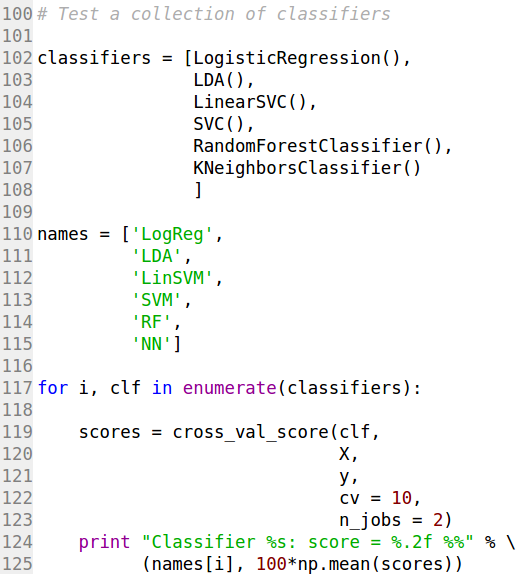
\includegraphics[width=1.0\columnwidth]{clf_loop_code.png}}}
{\scriptsize Result:}\\
\fbox{\centerline{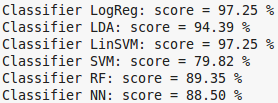
\includegraphics[width=0.8\columnwidth]{clf_loop_result.png}}}
\end{columns}
\end{frame}

\begin{frame}[fragile]{Selection of $K$ in cross-validation}
\begin{columns}
\column{0.7\textwidth}
\begin{itemize}
\item There is no definitive answer to the choice of number of folds in CV.
\item The best $K$ depends on the amount of data, difficulty of the problem,
error metric, etc.
\item In general, more folds is better, although the variance starts to increase
when approaching leave-one-out.
\item Attached is a figure of difference between CV error and true error
(which we happen to know in our artificial data case).
\end{itemize}
\column{0.3\textwidth}
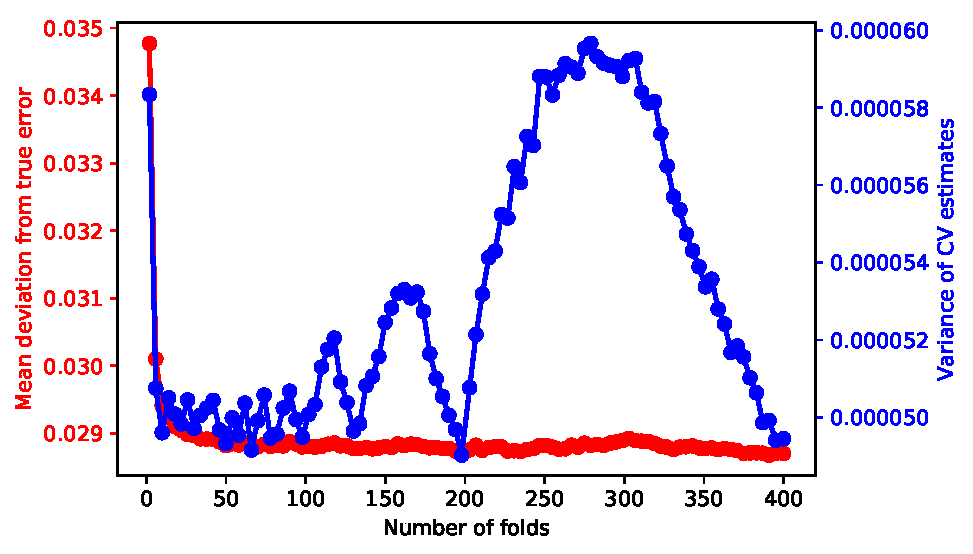
\includegraphics[width=1.0\columnwidth]{K_scores_var.pdf}\\

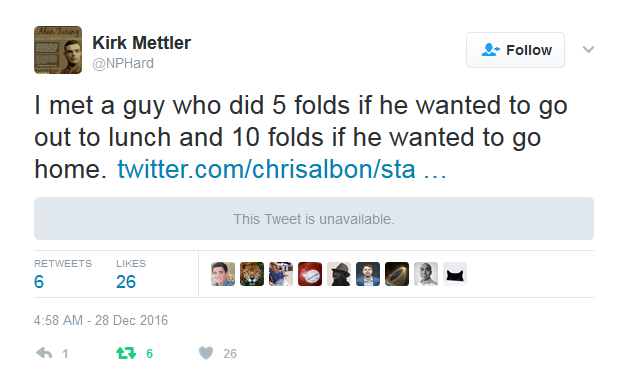
\includegraphics[width=\columnwidth]{folds_tweet.png}
\end{columns}
\end{frame}

\renewcommand{\leveys}{1.0\columnwidth}

\begin{frame}{Overfitting}
\begin{columns}
\column{0.75\textwidth}
\begin{itemize}
\item Generalization is also related to \emph{overfitting}.
\item On the right, a polynomial model is fitted to a time series to minimize the
error between the samples (red) and the model (green).
\item As the order of the polynomial increases, the model starts to follow the data 
very faithfully.
\item Low-order models do not have enough expression power.
\item High-order models are over-fitting to noise and become "unstable" with crazy values near the boundaries.
\end{itemize}
\column{0.25\textwidth}
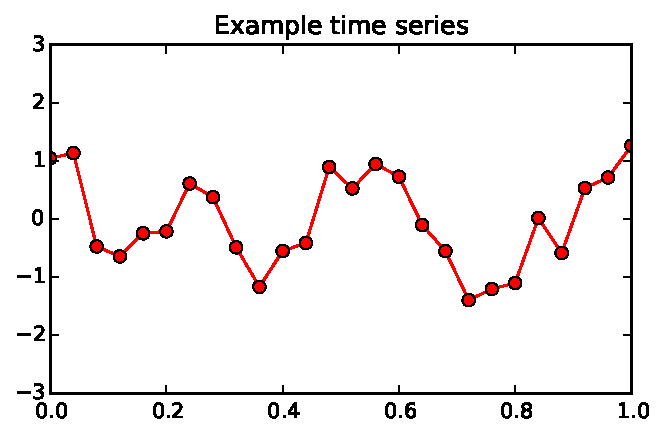
\includegraphics[width=\leveys]{timeSeries.pdf}\\
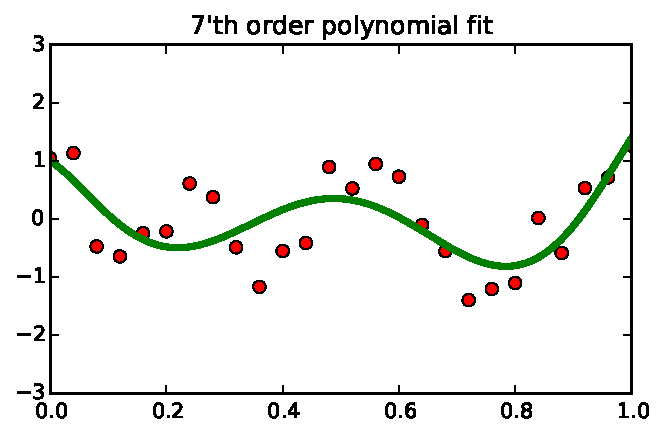
\includegraphics[width=\leveys]{timeSeries_7.pdf}\\
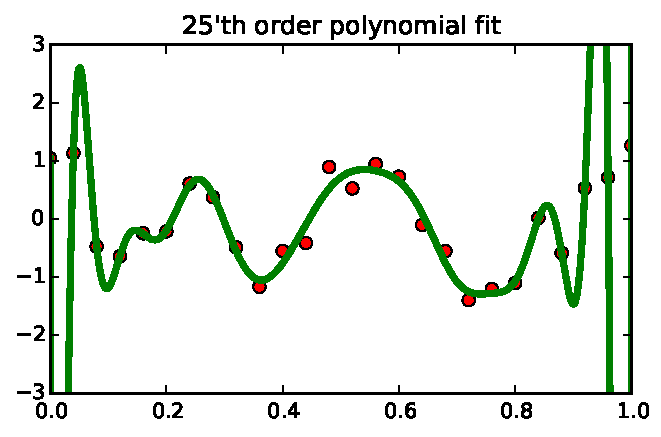
\includegraphics[width=\leveys]{timeSeries_25.pdf}
\end{columns}
\end{frame}


\begin{frame}{Regularization}
\begin{columns}
\column{0.75\textwidth}
\begin{itemize}
\item Regularization adds a penalty term to the fitting error.
\item The model is encouraged to use small coefficients.
\item Large coefficients are expensive, so the model can afford to fit only
to the major trends.
\item On the right, the high order model has a good expression power, but 
does still not follow the noise patterns.
\end{itemize}
\column{0.25\textwidth}
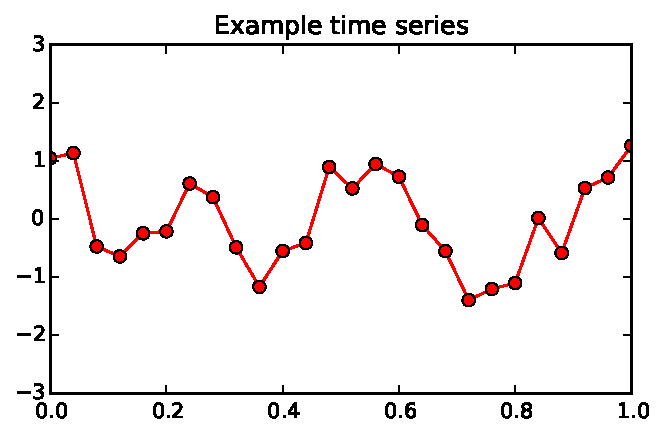
\includegraphics[width=\leveys]{timeSeries.pdf}\\
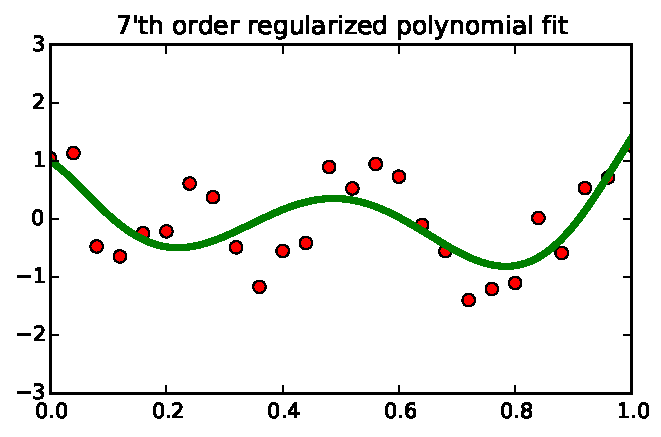
\includegraphics[width=\leveys]{timeSeries_7_reg.pdf}\\
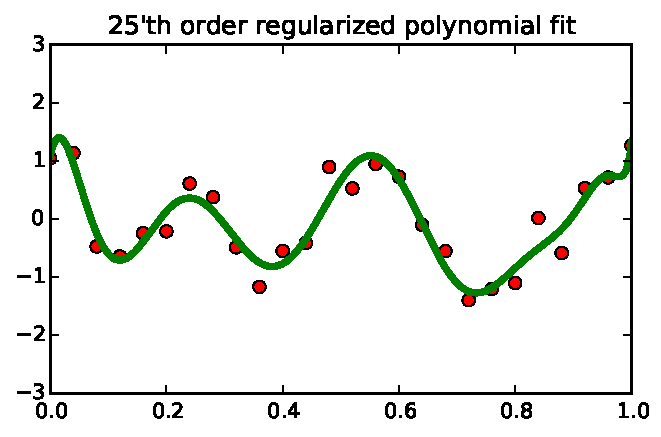
\includegraphics[width=\leveys]{timeSeries_25_reg.pdf}
\end{columns}
\end{frame}

\begin{frame}[fragile]{Regularization in Regression}
\begin{itemize}
\item Regularization techniques were first assessed in a regression context with linear models.
\item Linear regression model assumes that the inputs $\x_n\in \R^{P}$ and outputs $\y_n\in \R$ 
are related as
\[
y_n = \w^T\x_n + e_n,
\]
where $\e_n\sim {\cal N}(0, \sigma^2)$ is the error term.
\item With these assumptions, \emph{least squares} returns the optimal solution:
\[
\minimize_{\w}\left( \sum_{n = 0}^{N-1} (y_n - \w^T\x_n)^2 \right)
\]
\item There exists a closed form solution for LS:
\[
\w_{\text{LS}} = (\X^T\X)^{-1}\X^T\y.
\]
with $\X = \left[\x_0^T,\x_1^T,\ldots,\x_{N-1}^T\right]^T$.
\end{itemize}
\end{frame}

\begin{frame}[fragile]{Regularization in Regression}
\begin{itemize}
\item The most straightforward regularization technique adds a squared penalty with weight $\lambda>0$ for the weights:
\[
\minimize_{\w}\left( \sum_{n = 0}^{N-1} (y_n - \w^T\x_n)^2 + \lambda\w^T\w\right).
\]
\item This is called \emph{Tikhonov regularization} or \emph{Ridge Regression}, and there is a closed form solution:
\[
\w_{\text{RIDGE}} = (\X^T\X + \lambda{\bf I})^{-1}\X^T\y.
\]
\item Another name is $L_2$ regularization, because we take the $L_2$ norm of the weights.
\item In general, the $L_q$ norm (for $q>0$) is defined as 
\[
\|\w\|_q = \left( |w_0|^q +|w_1|^q + \cdots + |w_{P-1}|^{q} \right)^{-q}
\]
\item See \verb+sklearn.linear_model.Ridge+.
\end{itemize}
\end{frame}


\begin{frame}[fragile]{L1 Regularization in Regression}
\begin{itemize}
\item More recently, $L_1$ penalty has become popular---simply change the squared penalty into absolute penalty:
\[
\minimize_{\w}\left( \sum_{n = 0}^{N-1} (y_n - \w^T\x_n)^2 + \lambda\| \w\|_1 \right),
\]
with $\| \w \|_1 = \sum_p |w_p|$.
\item This is called \emph{LASSO penalty}\footnote{(Least Absolute Shrinkage and Selection Operator)}.
\item With this penalty, there is no closed form expression. 
\item The minimum is solved iteratively using, \emph{e.g.,} gradient search.
\item See \verb+sklearn.linear_model.Lasso+.
\end{itemize}
\end{frame}

\begin{frame}{$L_2$ Regularization with Linear Classifiers}
\begin{itemize}
\item The same regularizers apply also for linear classifiers.
\item \textbf{$L_2$ penalized Logistic Regression}:
\[
\text{penalized log-loss} = \sum_{n = 0}^{N-1}\underbrace{ \ln(1 + \exp(y_n\w^T\x_n))}_{\text {log-loss}} + \lambda \underbrace{\w^T\w}_{\text{penalty}}
\]
\item \textbf{$L_2$ penalized Linear SVM}:
\[
\text{penalized hinge loss} = \sum_{n = 0}^{N-1}\underbrace{ \max(0, 1-y_n\w^T\x_n)}_{\text {hinge loss}} + \lambda \underbrace{\w^T\w}_{\text{penalty}}
\]
\item The coefficient $\lambda\ge 0$ balances the strength of regularization:
\begin{itemize}
	\item Large $\lambda$: small coefficients (heavy penalty for large $\w^T\w$)
	\item Small $\lambda$: large coefficients (small penalty for large $\w^T\w$)
\end{itemize}
\end{itemize}
\end{frame}

\begin{frame}{$L_1$ Regularization with Linear Classifiers}
\begin{itemize}
	\item More recently, research has concentrated around the $L_1$ norm: $\|\w\|_1 = \sum |w_k|$.
\item \textbf{$L_1$ Regularized Logistic Regression}:
\[
\text{penalized log-loss} = \sum_{n = 0}^{N-1}\underbrace{ \ln(1 + \exp(y_n\w^T\x_n))}_{\text {log-loss}} + \lambda \underbrace{\|\w\|_1}_{L_1 \text{ penalty}}
\]
\item \textbf{$L_1$ Regularized Linear SVM}:
\[
\text{penalized log-loss} = \sum_{n = 0}^{N-1}\underbrace{ \max(0, 1-y_n\w^T\x_n)}_{\text {hinge loss}} + \lambda \underbrace{\|\w\|_1}_{L_1 \text{ penalty}}
\]
\end{itemize}
\end{frame}

\begin{frame}{Sparsity}
\begin{itemize}
\item A key benefit of $L_1$ is that it promotes \emph{sparse} weight vectors; \emph{i.e.,} most entries of $\w$ are zero.
\item This is equivalent to \textbf{feature selection:} most features are multiplied by zero, thus discarding them completely.
\item Feature selection property can be understood from an alternative formulation of the optimization problem.
\item The following two problems are equivalent
\[
\text{minimize} \sum_{n = 0}^{N-1} \ell(\w) + \lambda \|\w\|_p
\]
and
\[
\text{minimize} \sum_{n = 0}^{N-1} \ell(\w) \text{ such that } \|\w\|_p \le C
\]
with $\ell(\w)$ either the log loss or hinge loss and $p\in \{1,2\}$.
\end{itemize}
\end{frame}

\begin{frame}{Sparsity}
\begin{columns}
\column{0.7\textwidth}
\begin{itemize}
\item The parameters $\lambda$ and $C$ are obviously different. 
\item However, there is a one-to-one
mapping: for each $\lambda$ we can find the corresponding $C$ that gives the same solution.
\item In the latter formulation, we try to find the weight vector that 
minimizes the loss inside the region $\|\w\|_p \le C$.
\item This region is circular for $L_2$ and diamond shaped for $L_1$.
\item With $L_1$, the solutions are often at the corners of the diamond.
\end{itemize}
\column{0.3\textwidth}
\centerline{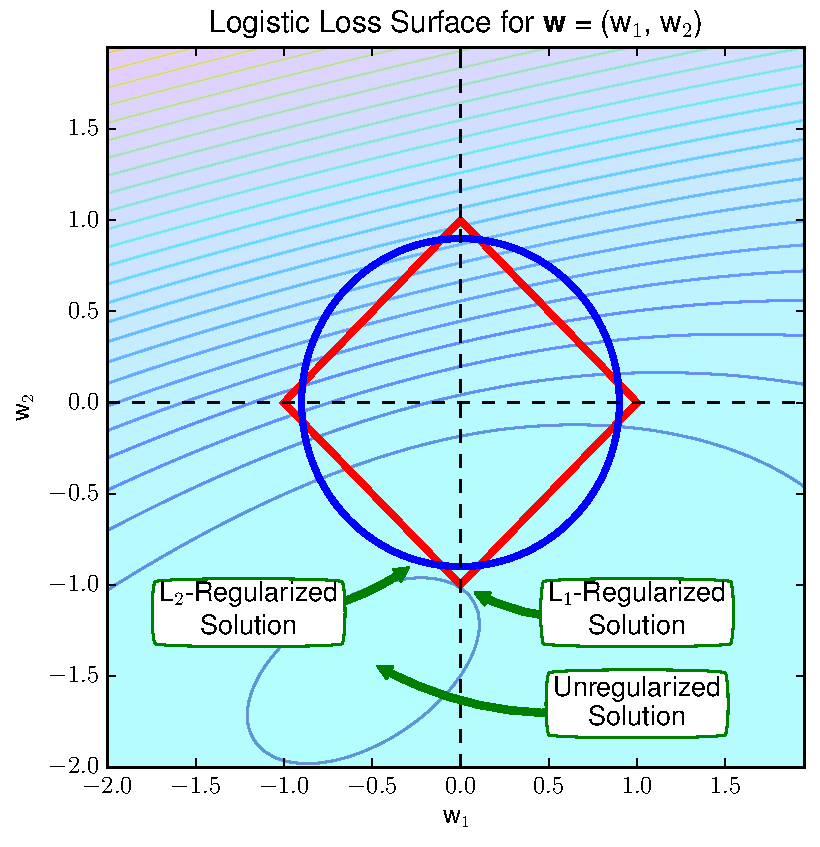
\includegraphics[width=\textwidth]{L1-reg.pdf}}

\vspace*{0.2cm}
{\small \em The $L_1$ solution tends to lie along the coordinate axes, where some of the coefficients are zero.

\vspace*{0.2cm}
This is more likely if the area size decreases (or $C\rightarrow 0$).\par}

\end{columns}
\end{frame}


\begin{frame}{Sparsity}
\begin{columns}
\column{0.4\textwidth}
\begin{itemize}
\item The plots illustrate the model coefficients without regularization,
with traditional regularization and sparse regularization.
\item The importance of sparsity is twofold: The model can be used for feature
selection, but often also generalizes better.
\end{itemize}
\column{0.3\textwidth}
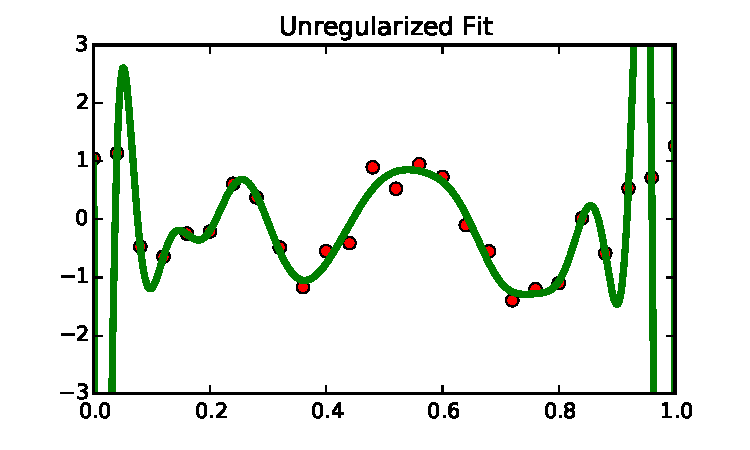
\includegraphics[width=\leveys]{unreg_fit.pdf}\\
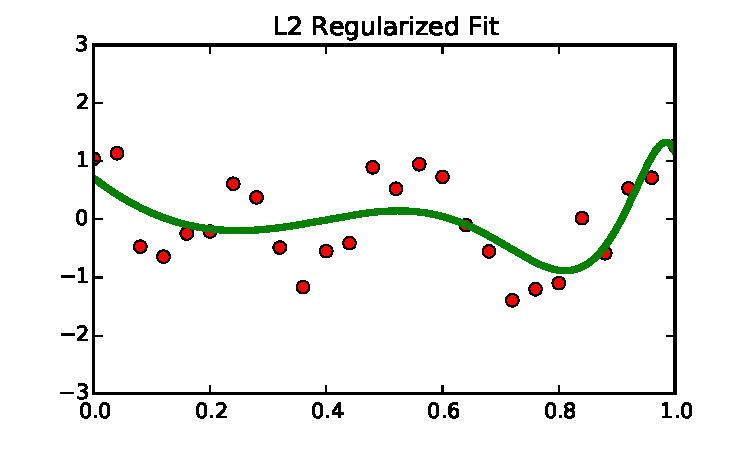
\includegraphics[width=\leveys]{L2_fit.pdf}\\
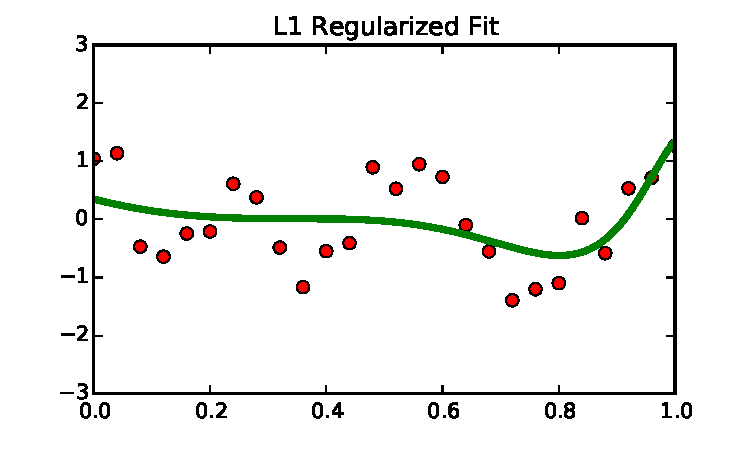
\includegraphics[width=\leveys]{L1_fit.pdf}
\column{0.3\textwidth}
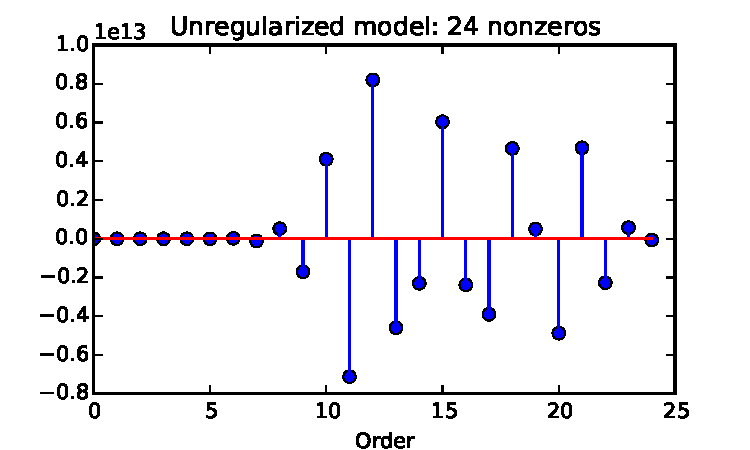
\includegraphics[width=\leveys]{unreg_coef.pdf}\\
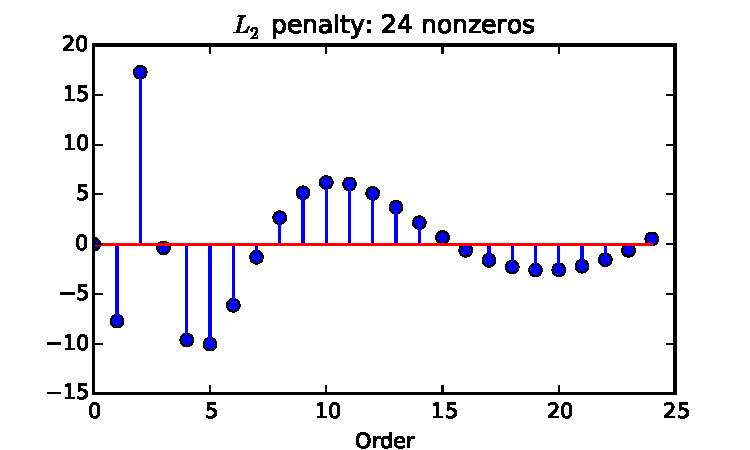
\includegraphics[width=\leveys]{RR_coef.pdf}\\
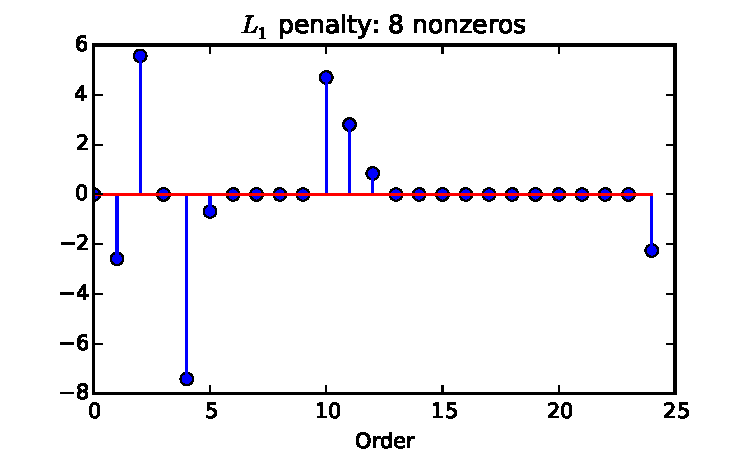
\includegraphics[width=\leveys]{lasso_coef.pdf}
\end{columns}
\end{frame}

\begin{frame}{Regularization in Ovarian Cancer Detection}
\begin{itemize}
\item We will study an example of classifying proteomic fingerprints of mass-spectra
measured from ovarian cancer patients and healthy controls.\footnote{\tiny Conrads, Thomas P., et al. "High-resolution serum proteomic features for ovarian cancer detection." \emph{Endocrine-Related Cancer} (2004).}
\item 121 cancer patients and 95 healthy controls.
\item Raw mass spectra consists of 10000 measurements.
\end{itemize}

\begin{center}
	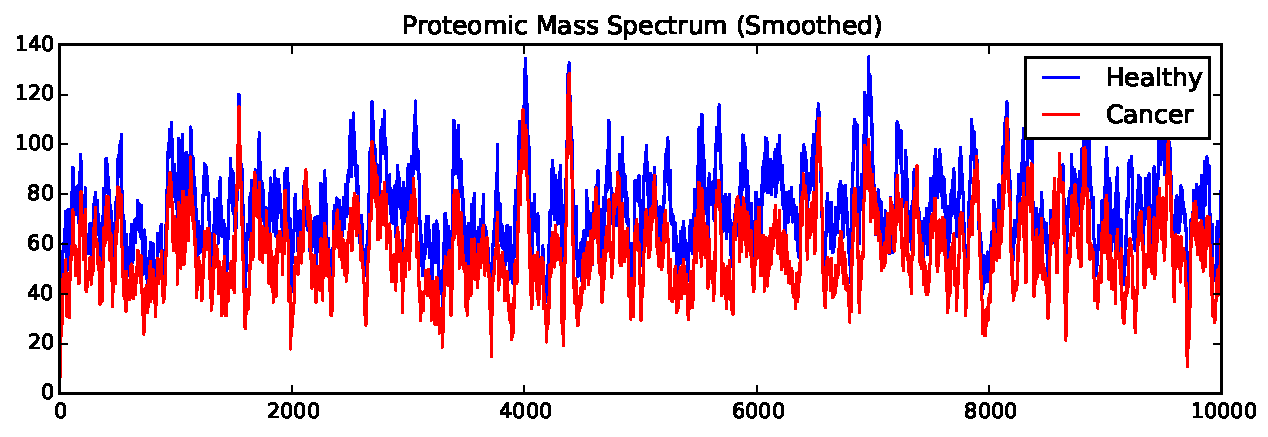
\includegraphics[width=0.5\columnwidth]{ovariancancer_plot.pdf}
\end{center}
\end{frame}

\begin{frame}[fragile]{Training a Classifier}
\begin{columns}[onlytextwidth]
\column{0.65\textwidth}
\begin{lstlisting}
classifiers = [(LogisticRegression(), "LogReg"),
               (LinearSVC(dual = False), "SVM")]
C_range = 10.0 ** np.arange(0,12, 0.25)

for clf, name in classifiers:

    for penalty in ["l1", "l2"]:            
        clf.penalty = penalty

        accuracies = []
        nonzeros = []

        for C in C_range:

            clf.C = C
            clf.fit(X_train, y_train)
            prediction = clf.predict(X_test)
            accuracy = 100.0 * np.mean(prediction == y_test)
\end{lstlisting}
\column{0.35\textwidth}
\begin{itemize}
\item The attached code trains and applies a LR and SVM
classifiers for the ovarian cancer problem.
\item We loop over two penalties and a range of regularization parameters $C$.
\end{itemize}
\end{columns}
\end{frame}



\begin{frame}[fragile]{Results}
\begin{center}
	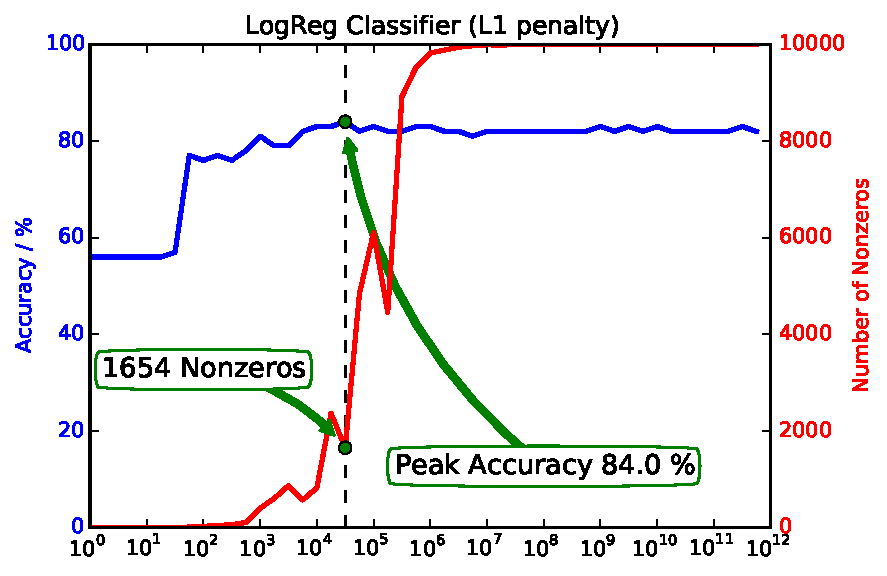
\includegraphics[width=0.35\textwidth]{ovarian_LogReg_l1.pdf}
	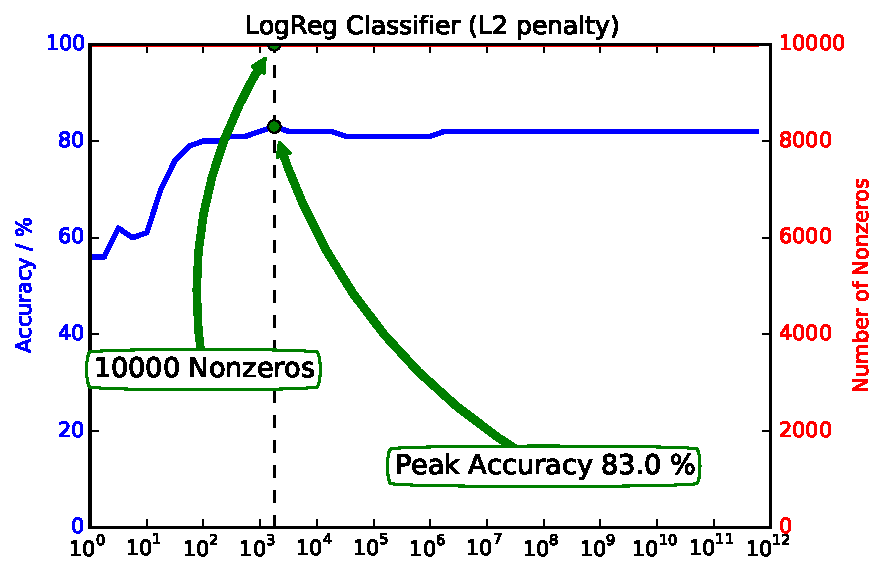
\includegraphics[width=0.35\textwidth]{ovarian_LogReg_l2.pdf}\\
	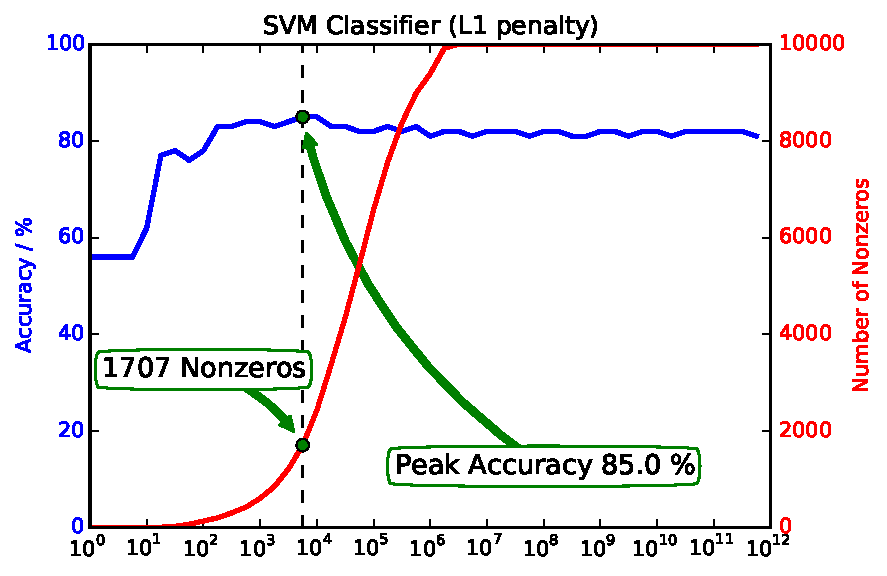
\includegraphics[width=0.35\textwidth]{ovarian_SVM_l1.pdf}
	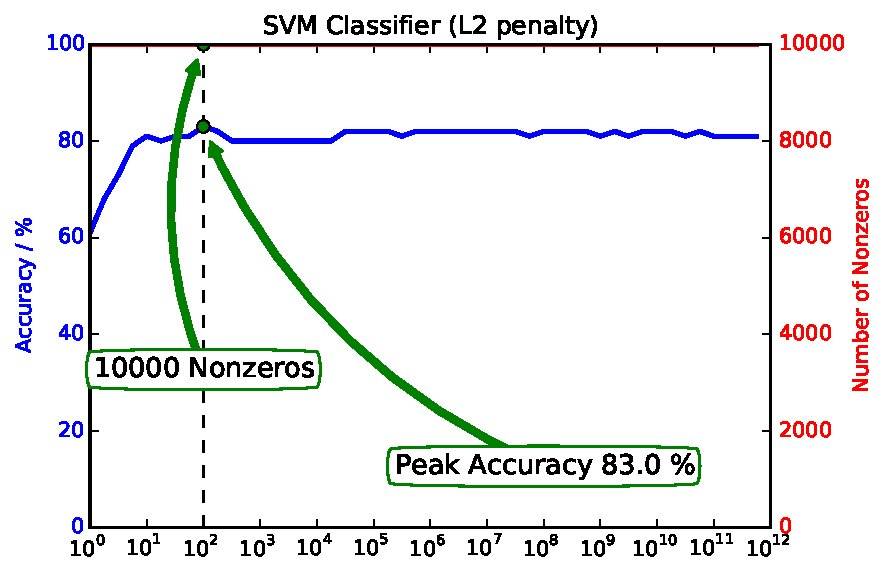
\includegraphics[width=0.35\textwidth]{ovarian_SVM_l2.pdf}	
\end{center}
\end{frame}


\begin{frame}[fragile]{Analysis of the Classifier}
\begin{columns}
\column{0.6\textwidth}
\begin{itemize}
\item The $\ell_1$ regularized Linear SVM was the
most accurate classifier.
\item It is defined by its coefficients $\w$.
\item The nonzero coefficients correspond to the
peaks of the mass spectra.
\end{itemize}
\column{0.4\textwidth}
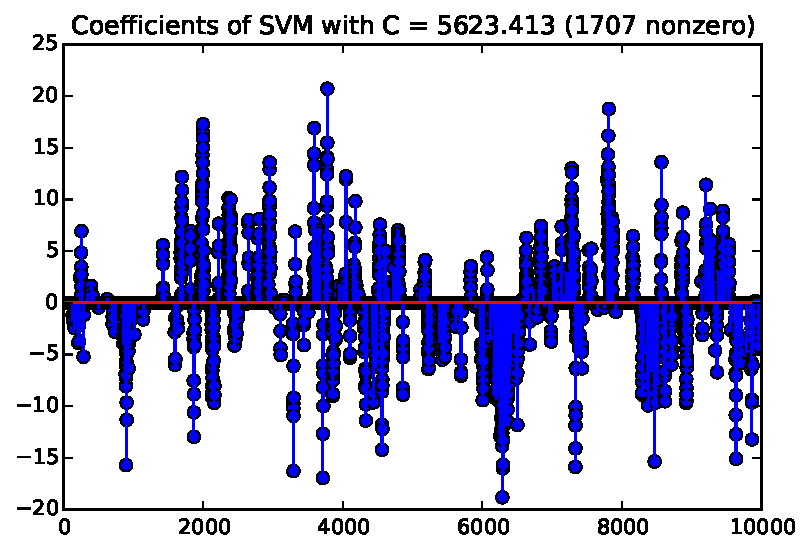
\includegraphics[width=1.1\columnwidth]{ovarian_coef.pdf}
\end{columns}
\end{frame}

\begin{frame}{Feature Selection}
\begin{itemize}
\item One of the benefits of $L_1$ regularization is its ability for \emph{feature selection}.
\item More specifically, $L_1$ can choose the most essential set of good features and discard the rest.
\item Helps in high-dimensional cases.
\item Improves performance by removing "confusers"; \emph{i.e.,} measurements which have no predictive value (or may even degrade performance).
\end{itemize}
\end{frame}

\begin{frame}[fragile,allowframebreaks=0.8]{Traditional Approaches to Feature Selection}
\begin{itemize}
\item \textbf{Variance based selection}: Retain features with high variance. 
\begin{itemize}
	\item Simple to implement; however: high variance may not imply importance.
	\item \verb+sklearn.feature_selection.VarianceThreshold+
\end{itemize}
\item \textbf{Statistics based selection}: Apply statistical tests for dependence between features and labels, \emph{e.g.,} chi-squared test.
\begin{itemize}
	\item Good if the assumptions are correct (often not the case).
	\item \verb+sklearn.feature_selection.SelectKBest+.
\end{itemize}
\item \textbf{Recursive selection}: Progressively add or remove features that seem to improve performance the most.
\begin{itemize}
	\item Forward selection starts with empty set and adds variables one by one.
	\item Backward elimination starts with full set and removes variables one by one.
	\item There are also hybrid versions that alternate between addition and removal.
	\item \verb+sklearn.feature_selection.RFECV+ implements this (with cross-validation).
\end{itemize}
\end{itemize}
\end{frame}

\begin{frame}[fragile,allowframebreaks=0.8]{Example}
\begin{columns}
\column{0.8\textwidth}
\begin{itemize}
\item Consider an example of classifying the \emph{digits} dataset (\verb+sklearn.datasets.load_digits+).
\item We use LDA classifier with recursive feature elimination.
\item For simplicity, we consider only two classes (zeros and ones).
\end{itemize}
\begin{lstlisting}
from sklearn.datasets import load_digits
from sklearn.lda import LDA
from sklearn.feature_selection import RFECV

digits = load_digits()

# Use only classes 8 and 9
X = digits.data[digits.target > 7, :]
y = digits.target[digits.target > 7]

# Select features
rfecv = RFECV(estimator=LDA())
rfecv.fit(X, y)

# Scores and feature sets are here
scores = rfecv.grid_scores_
mask = rfecv.support_.reshape(8, 8)
\end{lstlisting}

\column{0.18\textwidth}
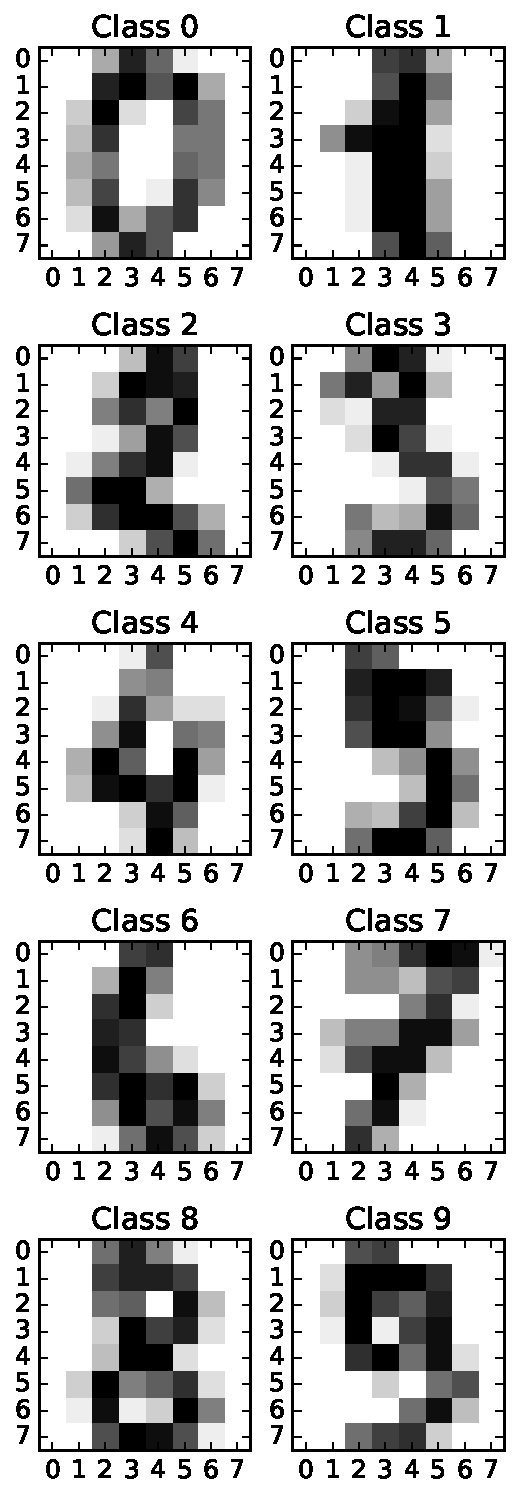
\includegraphics[width=\textwidth]{digits.pdf}
\end{columns}
\end{frame}

\begin{frame}{Results}
\begin{itemize}
\item The smallest high scoring set of features consists of 43 pixels.
\item There are also larger sets with equal score.
\item However, using all features will give a lower score.
\end{itemize}
\begin{center}
	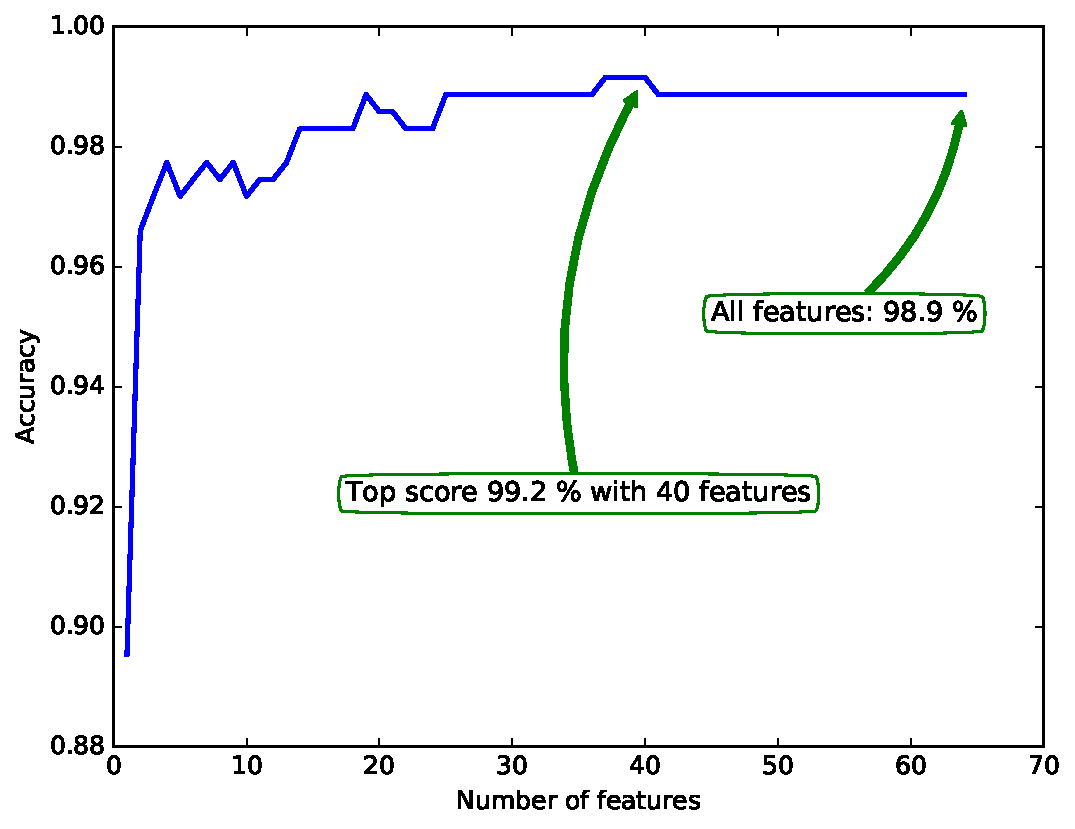
\includegraphics[height=0.4\textheight]{rfe_accuracy.pdf}
\qquad
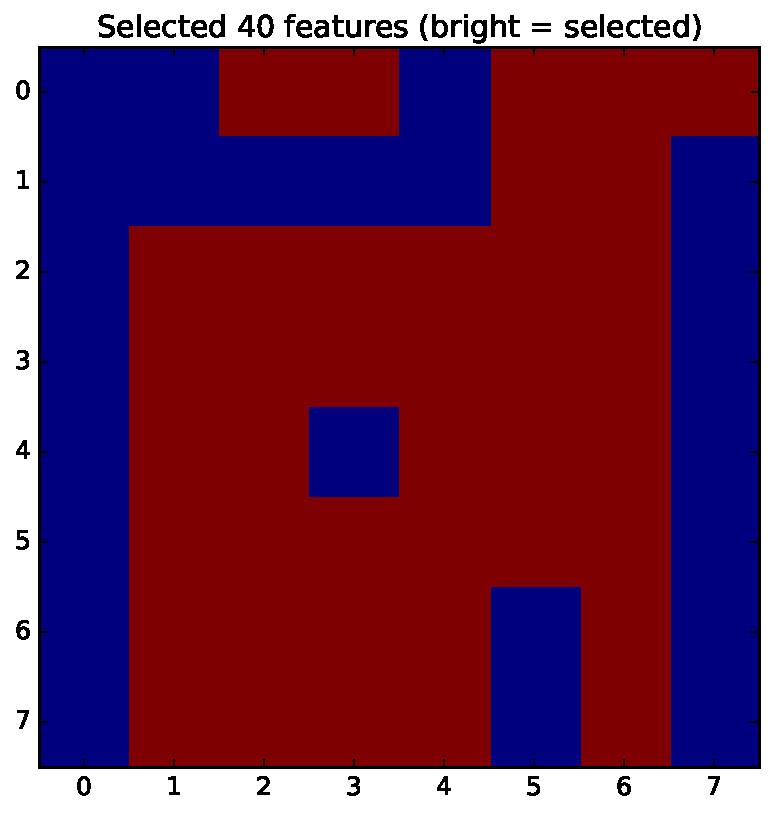
\includegraphics[height=0.4\textheight]{rfe_mask.pdf}
\end{center}
\end{frame}

\begin{frame}[fragile,allowframebreaks=0.8]{Example with L1-LR}
\begin{columns}
\column{0.8\textwidth}
\begin{itemize}
\item Let's try to use $L_1$ regularized logistic regression for the same task.
\end{itemize}
\begin{lstlisting}
from sklearn.datasets import load_digits
from sklearn.linear_model import LogisticRegression
from sklearn.model_selection import cross_val_score

digits = load_digits()

# Use only classes 8 and 9
X = digits.data[digits.target > 7, :]
y = digits.target[digits.target > 7]

# Select features
clf = LogisticRegression(penalty = "l1")
C_range = 10.0 ** np.arange(-5,6, 0.5)

accuracies = []
nonzeros = []
bestScore = 0

for C in C_range:
    clf.C = C
    score = cross_val_score(clf, X, y, cv = 5).mean()    
\end{lstlisting}
\column{0.18\textwidth}
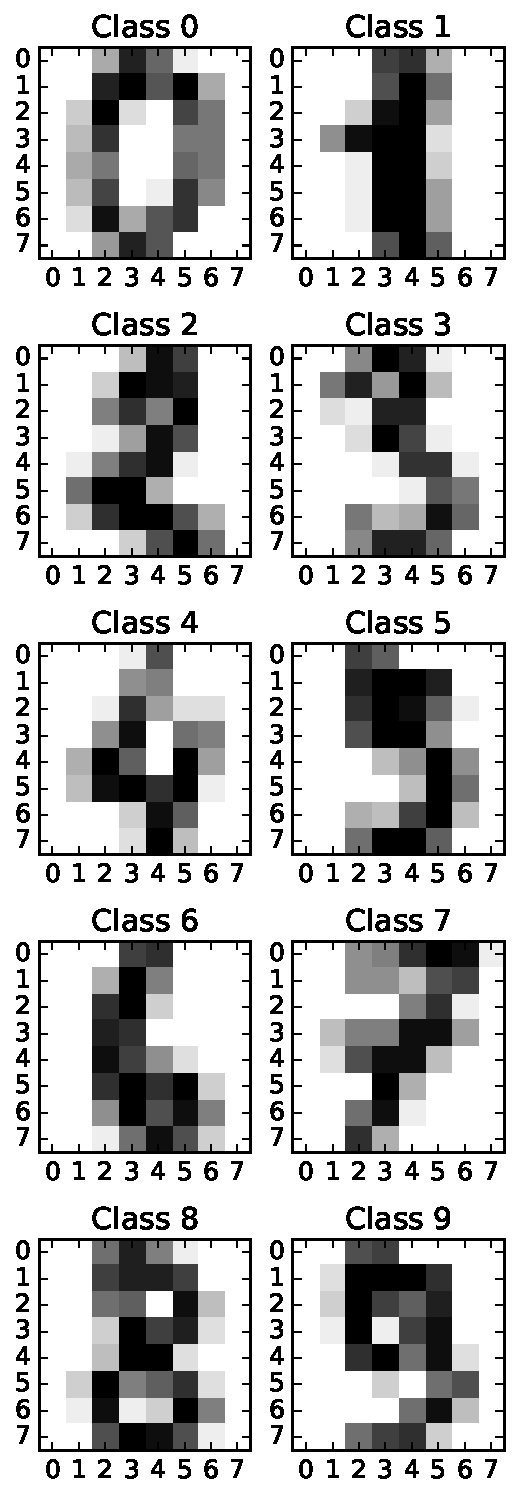
\includegraphics[width=\textwidth]{digits.pdf}
\end{columns}
\end{frame}

\begin{frame}{Example}
\begin{itemize}
\item The smallest high scoring set of features consists of 50 pixels.
\item Note: a different set will result at each run due to randomness of CV-5. Also the below set is different from the CV results---trained with all data.
\item The $L_1$ feature set seems 'better' than RFE.
\end{itemize}
\begin{center}
	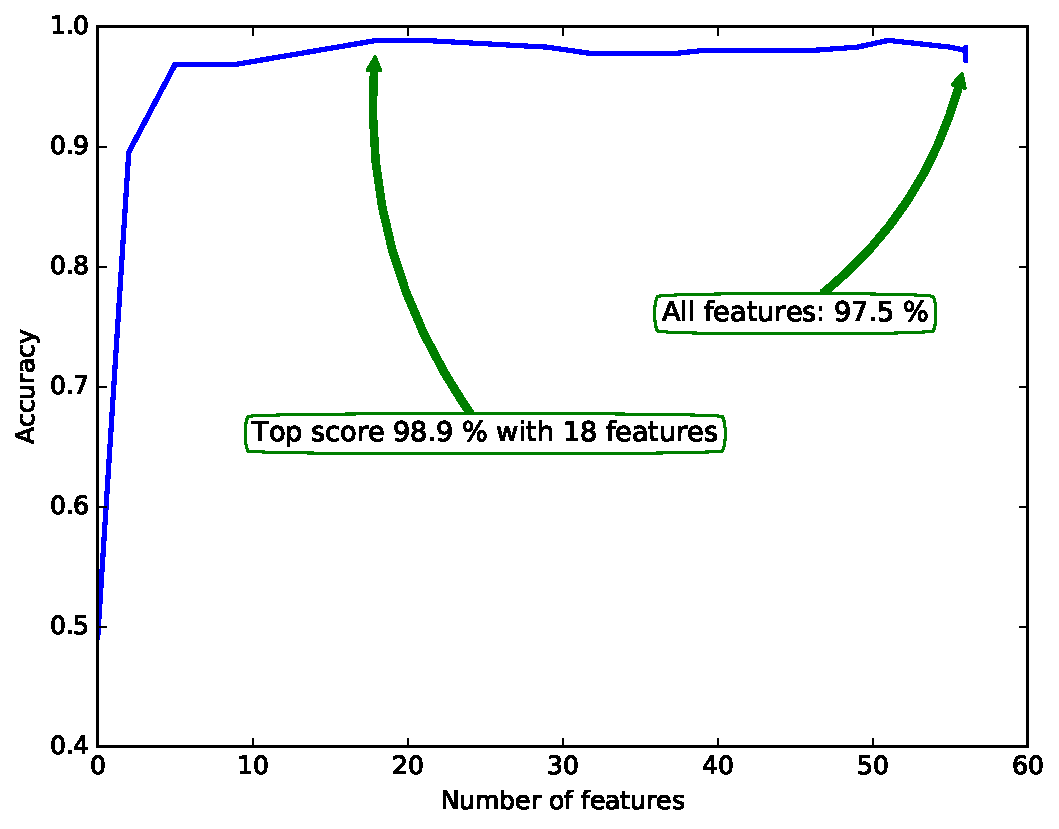
\includegraphics[height=0.4\textheight]{L1_digits_accuracy.pdf}
\qquad
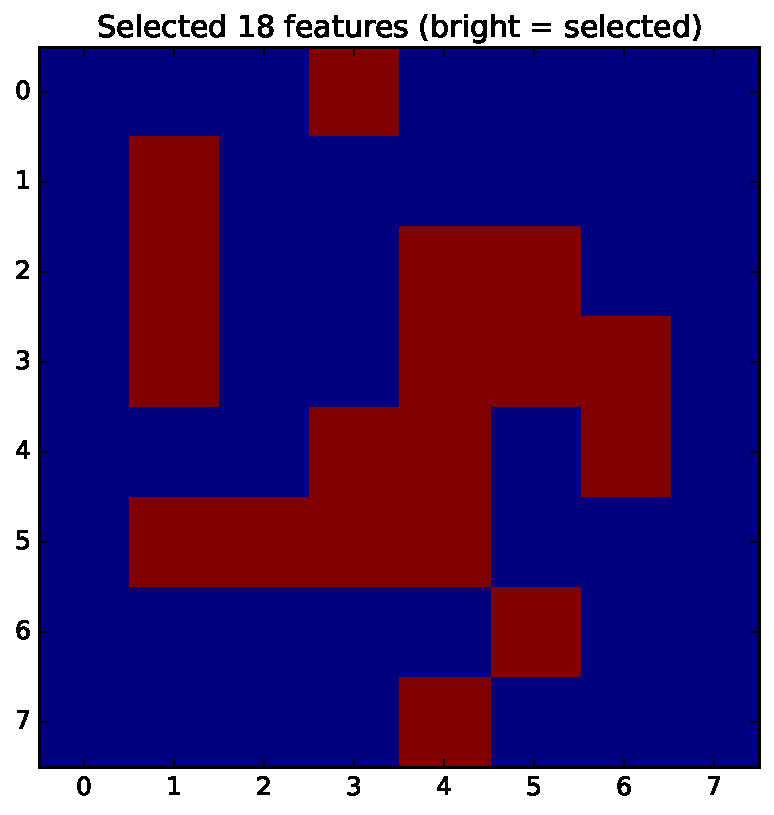
\includegraphics[height=0.4\textheight]{L1_digits_mask.pdf}
\end{center}
\end{frame}


\begin{frame}[fragile]{Randomized LogReg for Feature Selection}
\begin{itemize}
\item Basic $L_1$ feature selection has been extended through randomization.
\item The randomized version iterates by showing subsamples of the training set and observes
which features get selected consistently.
\item More robust than normal $L_1$; also called \emph{stability selection}.
\item See \verb+sklearn.linear_model.RandomizedLogisticRegression+ for classification.
\item See \verb+sklearn.linear_model.RandomizedLasso+ for regression.
\end{itemize}
\end{frame}

\begin{frame}[fragile]{Example}
\begin{columns}[onlytextwidth]
\column{0.63\textwidth}
\begin{lstlisting}
from sklearn.linear_model import RandomizedLogisticRegression

# Train the model 1000 times, always sampling 75% of all data
# After 1000 runs, the feature is chosen if it appears
# in at least 25% of the feature sets.
# C is the L1 regularization parameter for LogReg.

model = RandomizedLogisticRegression(C = 1, 
                                     sample_fraction = 0.75,
                                     n_resampling = 1000,
                                     selection_threshold=0.25,
                                     n_jobs = 2,
                                     random_state = 42)
                        
model.fit(X, y)
mask = model.get_support() # 64 binary variables.
mask = mask.reshape(8,8) 
\end{lstlisting}
\column{0.37\textwidth}
\begin{itemize}
\item The benefit of Randomized LogReg is its stability.
\item The selected features are very similar on different test runs.
\end{itemize}
\begin{center}
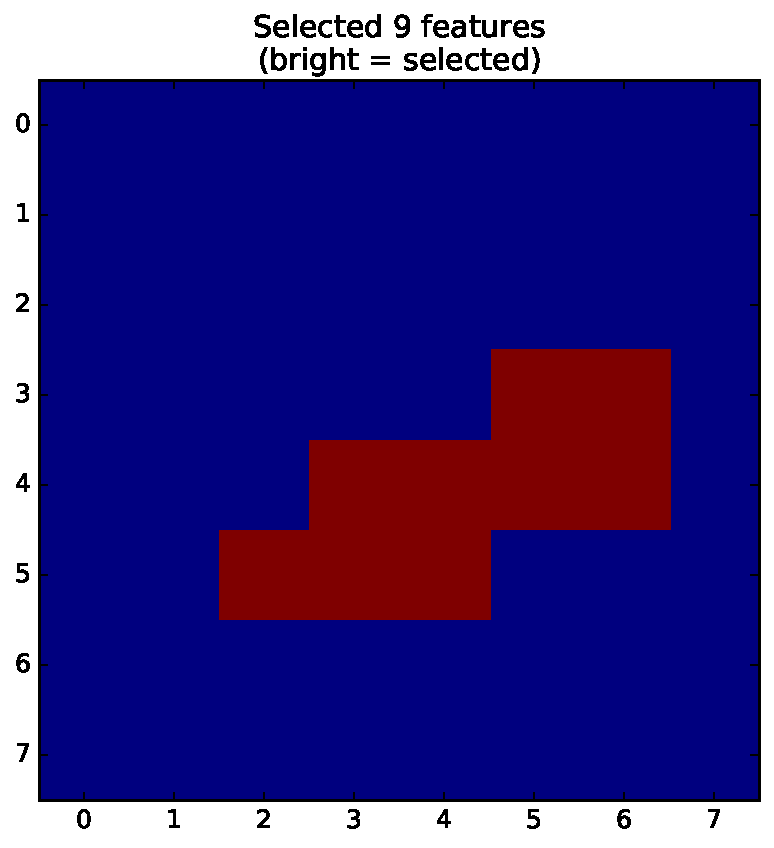
\includegraphics[width=0.7\columnwidth]{Stability_selection_digits_mask.pdf}
\end{center}
\end{columns}
\end{frame}

\begin{frame}[fragile]{Feature Ranking}
\begin{columns}
\column{0.85\textwidth}
\begin{itemize}
	\item Often, we are interested in the relative importance of features---not only which where selected, but in which order.
	\item Random forest derives this by shuffling each feature and studying the effect in accuracy: \verb+RandomForestClassifier.feature_importances:+.
	\item Randomized Logistic Regression keeps track of how often each feature was selected: \verb+RandomizedLogisticRegression.scores_+.
	\item Also, the RFECV keeps track of the order in which features were dropped: \verb+RFECV.ranking_+.
	\item The plots for our data are shown on the right.
\end{itemize}
\column{0.15\textwidth}
\begin{center}
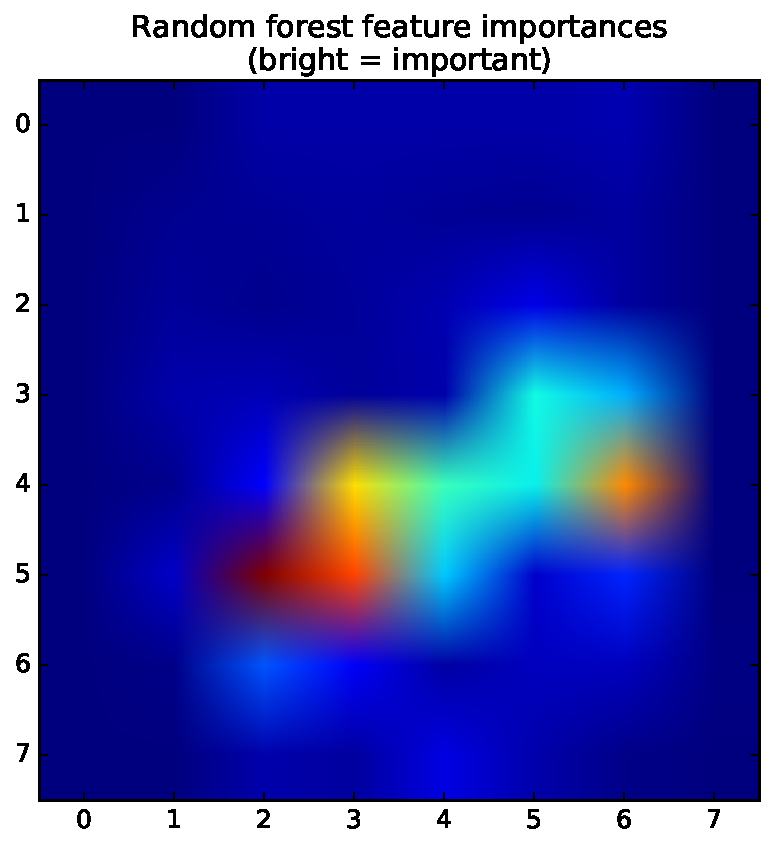
\includegraphics[width=\columnwidth]{RF_ranking.pdf}\\
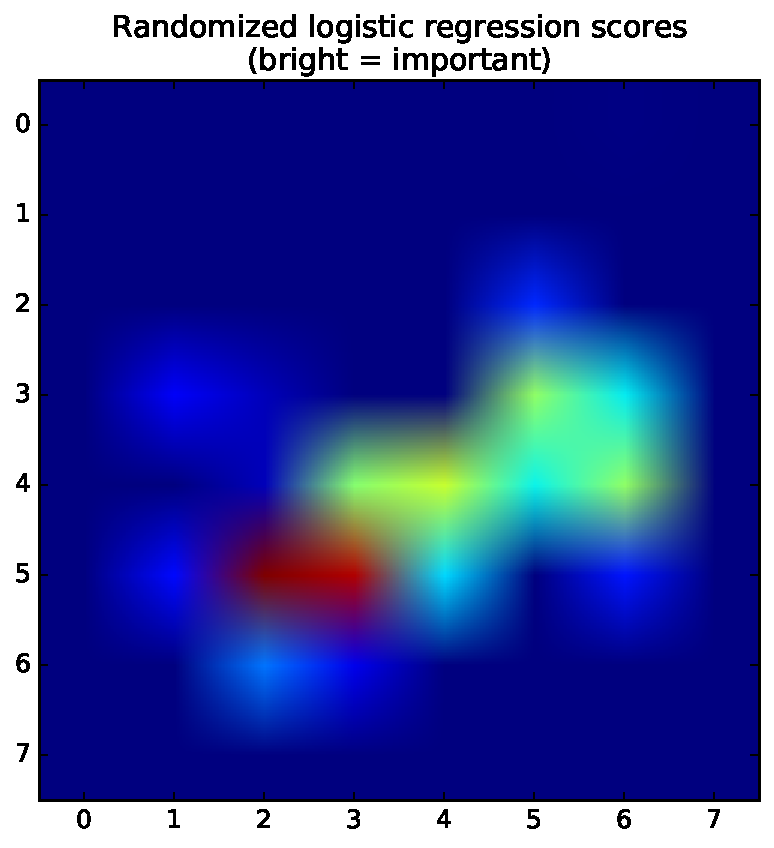
\includegraphics[width=\columnwidth]{RLR_ranking.pdf}\\
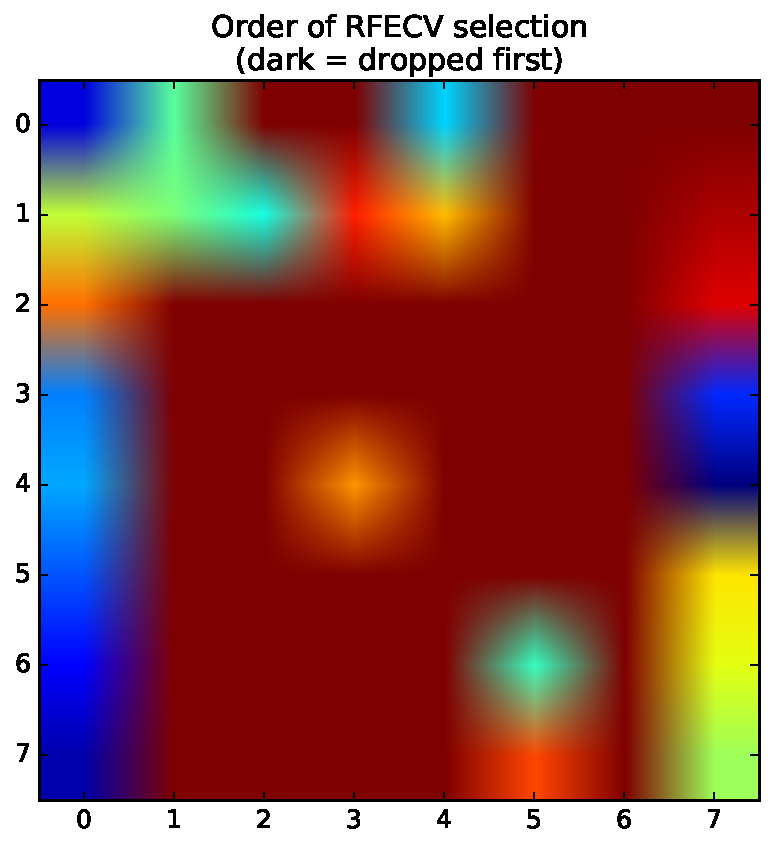
\includegraphics[width=\columnwidth]{RVECF_ranking.pdf}
\end{center}
\end{columns}
\end{frame}

\begin{frame}[fragile]{Unsupervised learning}
	\begin{itemize}
		\item Unsupervised learning does not require class labels, but instead attempts to understand the data without them.
		\item Unsupervised learning has many uses, such as:
			\begin{enumerate}
				\item Finding clusters within the data
				\item Transforming the data representation more suitable for later use; \emph{e.g.}, dimensionality reduction
			\end{enumerate}
			\item Let's study each of them in more detail.
	\end{itemize}
\end{frame}

\begin{frame}[fragile, allowframebreaks=0.8]{Clustering}
		\begin{columns}
		\column{0.6\textwidth}
	    \begin{itemize}
			\item K-means is a standard algorithm for splitting unlabeled data into clusters.
			\item K-means requires the number of assumed clusters as input.
	    \end{itemize}
			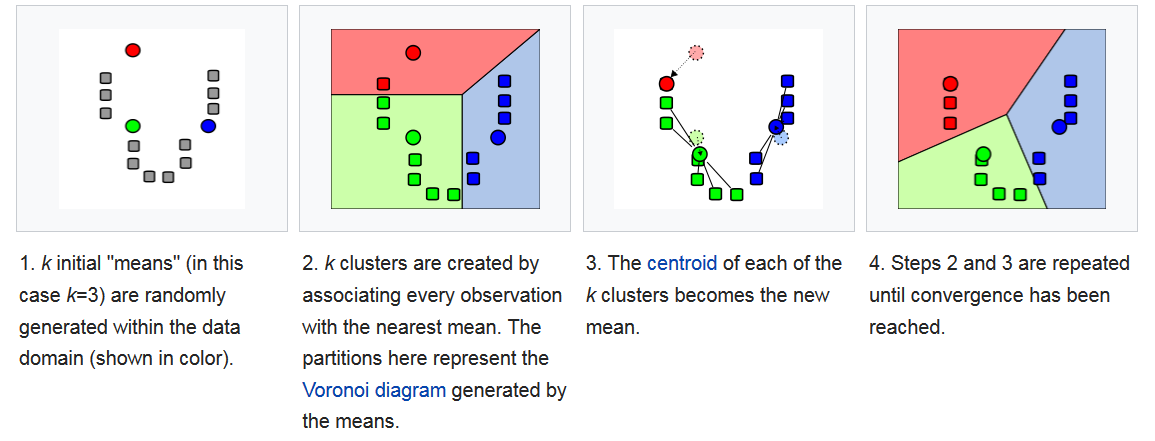
\includegraphics[width=\columnwidth]{K_means.png}
			
			\emph{\scriptsize Figure credits: Wikipedia::K-means clustering}
	  \column{0.4\textwidth}
		\begin{center}
			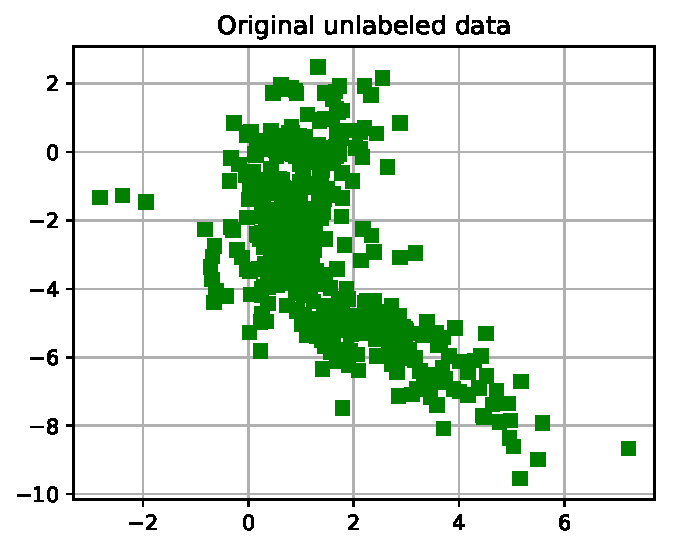
\includegraphics[width=0.5\columnwidth]{kmeans_orig.pdf}
			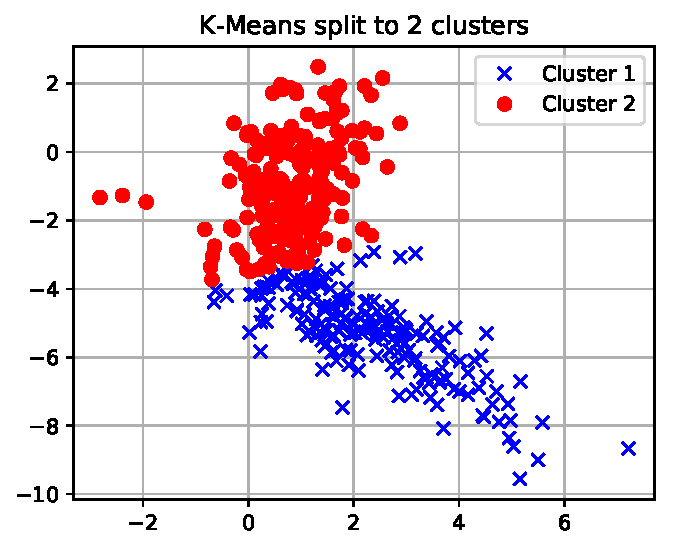
\includegraphics[width=0.5\columnwidth]{kmeans_2.pdf}\\
			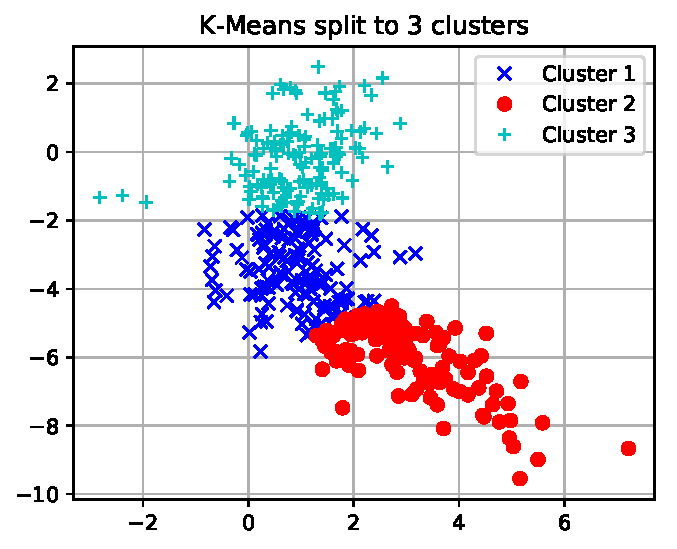
\includegraphics[width=0.5\columnwidth]{kmeans_3.pdf}
			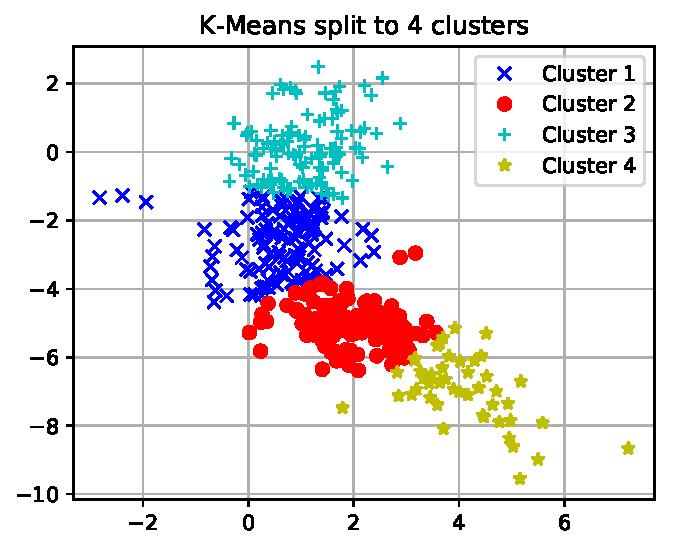
\includegraphics[width=0.5\columnwidth]{kmeans_4.pdf}\\
			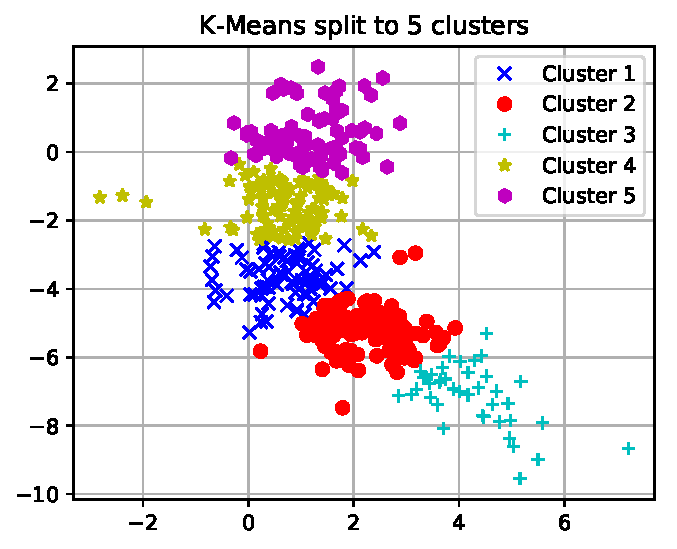
\includegraphics[width=0.5\columnwidth]{kmeans_5.pdf}
			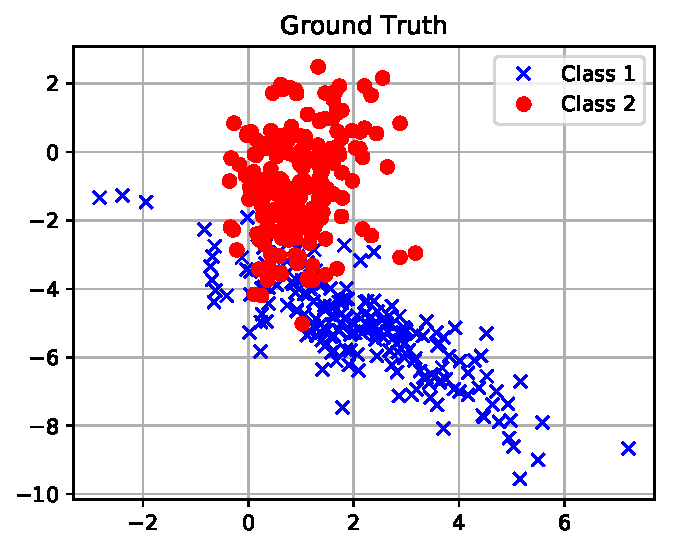
\includegraphics[width=0.5\columnwidth]{kmeans_true.pdf}
		\end{center}
		\end{columns}
\end{frame}

\begin{frame}[fragile, allowframebreaks=0.8]{Dimensionality reduction}
		\begin{columns}
		\column{0.7\textwidth}
	    \begin{itemize}
			\item High dimensional data may have a lot of redundancy (correlation) between features.
			\item This can be compressed by mapping to a lower dimension while preserving most of the variation.
			\item \textbf{Principal component analysis} (PCA) is a classical approach for this.
			\item PCA finds the directions, where the data has maximum variation.
			\item In the figure, the first principal component (PC) is the direction with highest variance.
			\item The second PC is the next (orthogonal direction) with second highest variance.
	    \end{itemize}
			
	  \column{0.3\textwidth}
		\begin{center}
			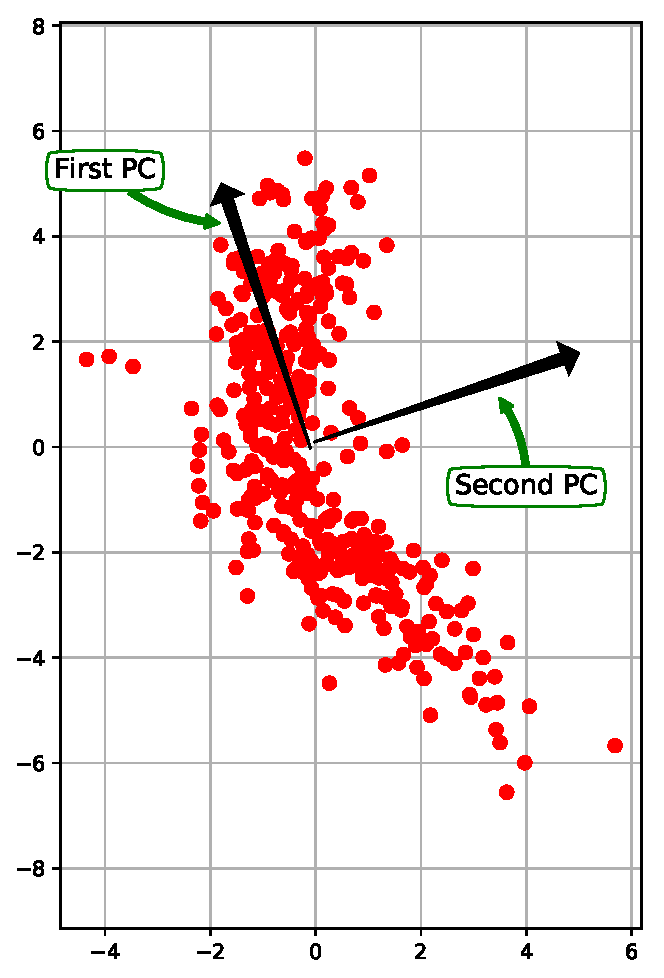
\includegraphics[width=\columnwidth]{PCA_example.pdf}
		\end{center}
		\end{columns}
\end{frame}

\begin{frame}[fragile, allowframebreaks=0.8]{The PCA}
	    \begin{itemize}
			\item It can be shown that the PCA axes are eigenvectors of  covariance matrix:
			\[
			{\bf V} = \text{eig}({\bf X}^T{\bf X})
			\]
\end{itemize}
		\begin{columns}
		\column{0.75\textwidth}
	    \begin{itemize}
			\item In numpy terms, this is only one line of code.
\begin{lstlisting}
from numpy.linalg import eig
from numpy import cov

# Assume our data is in X with shape [400, 2].
D, V = eig(cov(X, rowvar = False))

print("First PC: %s" % str(V[:, 0]))
print("Second PC: %s" % str(V[:, 1]))   
\end{lstlisting}

\begin{lstlisting}
First PC: [-0.33683673  0.94156307]
Second PC: [ 0.94156307  0.33683673]
\end{lstlisting}
\item Note: the PC's may not be in the order of decreasing variance.
 Use eigenvalues \verb+D+ to reorder: 
\verb+V = V[:, np.argsort(D)]+. Then, \verb+V[:, -1]+ will be the 1st PC.
\end{itemize}
			
	  \column{0.25\textwidth}
		\begin{center}
			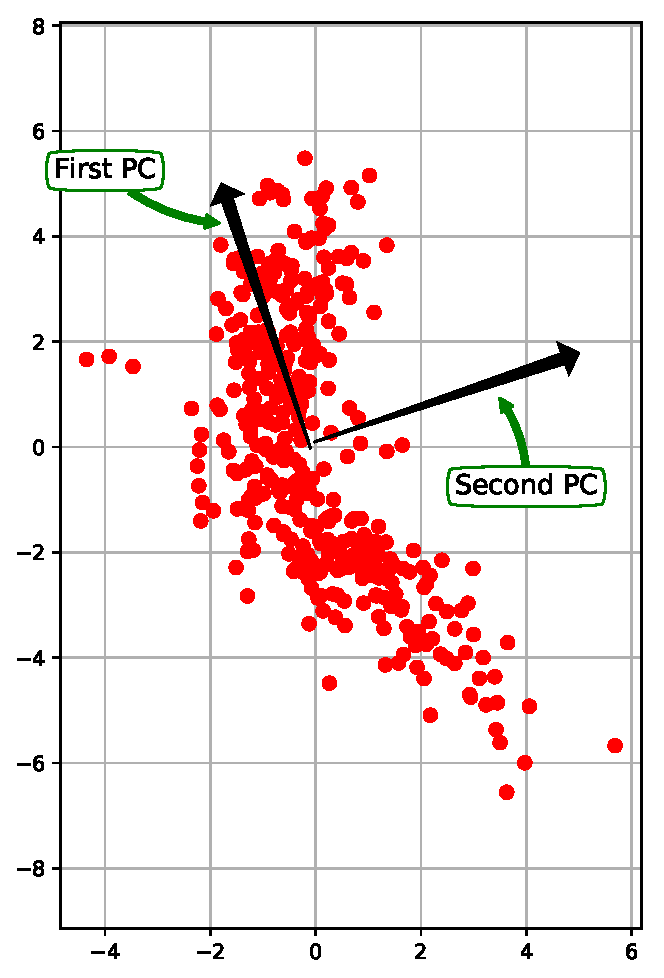
\includegraphics[width=\columnwidth]{PCA_example.pdf}
		\end{center}
		\end{columns}
\end{frame}

\begin{frame}[fragile, allowframebreaks=0.8]{Understanding the PCA}
		\begin{columns}
		\column{0.75\textwidth}
	    \begin{itemize}
\item The matrix \verb+V+ of previous slide transforms the data to a new coordinate system.
\item In other words, multiplication by \texttt{V} only rotates the coordinate axes.
\item Below we fit a PCA into the 64-dimensional digits dataset.
\begin{lstlisting}
from sklearn.datasets import load_digits

digits = load_digits()
X = digits.data

# Compute 64x64 PCA matrix V:
D, V = eig(cov(X, rowvar = False))

# Subtract mean from each column:
X = X - np.tile(X.mean(axis = 0), [X.shape[0], 1])

# Map X through the PCA (rotate axes):
X_rot = np.matmul(X, V)

\end{lstlisting}

\end{itemize}
			
	  \column{0.25\textwidth}
		\begin{center}
		  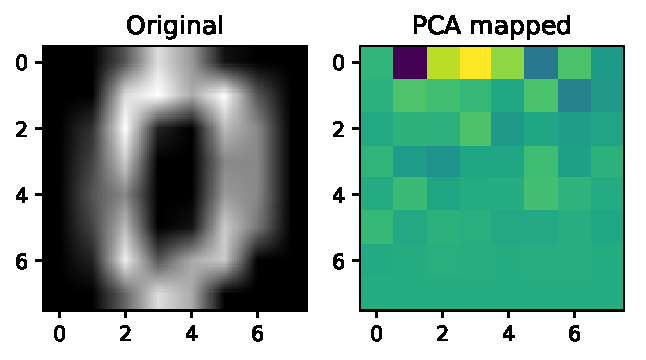
\includegraphics[width=\columnwidth]{digits_pca_proj_example1.pdf}\\
			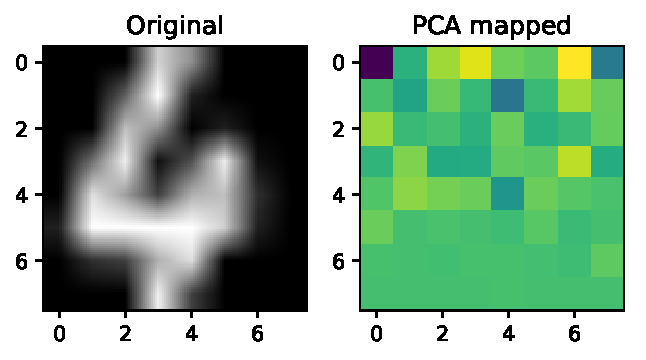
\includegraphics[width=\columnwidth]{digits_pca_proj_example2.pdf}\\
			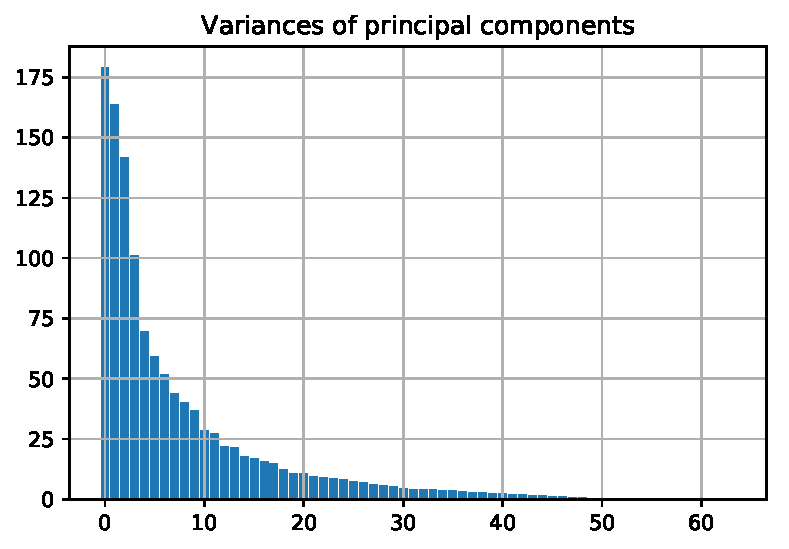
\includegraphics[width=\columnwidth]{digits_pca_proj_vars.pdf}
		\end{center}
		\end{columns}
\end{frame}


\begin{frame}[fragile, allowframebreaks=0.8]{PCA in Dimensionality Reduction}
		\begin{columns}
		\column{0.7\textwidth}
	    \begin{itemize}
\item The first 2 principal components cover 28.5 \% of all variance.
\item So maybe they also contain most of the information of the bitmaps.
\item Let's see how the 2 components reside in the 2D space.
\begin{lstlisting}
# Assume X_rot contains the PCA of previous slide.

# Retain only 2 components and plot
X_2D = X_rot[:, :2]

labels = ['zeros', 'ones', 'twos', 'threes', 'fours', 'fives', 'sixes', 'sevens', 'eights', 'nines']

for k in range(10):
    plt.scatter(X_2D[y == k, 0], X_2D[y == k, 1], label = labels[k])

plt.legend(loc = 'best')
\end{lstlisting}

\end{itemize}
			
	  \column{0.3\textwidth}
		\begin{center}
			\includegraphics[width=\columnwidth]{digits_pca_proj.pdf}
		\end{center}
		\end{columns}
\end{frame}

\begin{frame}[fragile, allowframebreaks=0.8]{Eigenimages}
		\begin{columns}
		\column{0.8\textwidth}
	    \begin{itemize}
\item The first principal components represent templates, against which we correlate each frame.
\item How do these \emph{eigenimages} look like?
\begin{lstlisting}
fig, ax = plt.subplots(4, 2, figsize = [3,7])

for k in range(4):
    for j in range(2):
        ax[k][j].imshow(V[:, k].reshape(8,8))
        ax[k][j].set_title("Eigenimage %d" % (k * 2 + j + 1))
\end{lstlisting}

\end{itemize}
			
	  \column{0.2\textwidth}
		\begin{center}
			\includegraphics[width=\columnwidth]{digits_eigenimages.pdf}
		\end{center}
		\end{columns}
\end{frame}

\begin{frame}[fragile, allowframebreaks=0.8]{PCA in Classification}
		\begin{columns}
		\column{0.6\textwidth}
	    \begin{itemize}
\item Let's try to classify the arcene dataset with PCA dimensionality reduction.

\begin{lstlisting}
from sklearn.discriminant_analysis import LinearDiscriminantAnalysis
from sklearn.metrics import accuracy_score
from sklearn.decomposition import PCA
	
# Remove Mean
normalizer = Normalizer()
normalizer.fit(X_train)
X_train = normalizer.transform(X_train)
X_test  = normalizer.transform(X_test)	

# Use sklearn PCA, because it is faster.
pca = PCA()
pca.fit(X_train)
X_train = pca.transform(X_train)
X_test  = pca.transform(X_test)

accuracies = []

for num_components in range(1, 100):
    clf = LinearDiscriminantAnalysis()
    clf.fit(X_train[:, :num_components], y_train)    
    y_pred = clf.predict(X_test[:, :num_components])    
    accuracy = accuracy_score(y_test, y_pred)
    accuracies.append(accuracy)
\end{lstlisting}

\end{itemize}
			
	  \column{0.4\textwidth}
		\begin{center}
			\includegraphics[width=\columnwidth]{arcene_pca.pdf}
		\end{center}
		\end{columns}
\end{frame}


\begin{frame}{Hyperparameter Optimization}
	\begin{itemize}
		\item The most common hyperparameter optimization techniques are:
		\begin{enumerate}
			\item \textbf{Grid search:} Try each hyperparameter combination in a fixed grid. For example, try SVM with 
			kernels 'linear' and 'rbf' and with C = [1,10,100,1000] (total 8 combinations).
			\item \textbf{Random search:} Randomize the hyperparameters. For example, select the kernel at
			random from \{'linear', 'rbf'\} and C from the range [1, 1000]. Iterate $N$ times.
			\item \textbf{Optimized grid search:} Instead of trying all combinations on a fixed grid, try
			to cover the search space as uniformly as possible.
			\item \textbf{Reactive search:} Use the results of previous iterations for choosing the next hyperparameter combination.
			For example, previous iterations suggest that 'rbf' gives better scores than 'linear', so it is
			favored in subsequent trials.
		\end{enumerate}
	\end{itemize}
\end{frame}

\begin{frame}[fragile]{Grid Search}
\begin{columns}[onlytextwidth]
\column{0.63\textwidth}
\begin{lstlisting}
from sklearn.grid_search import GridSearchCV
from sklearn.svm import SVC

# Define two grids; for linear and rbf
grid1 = {'kernel': ['linear'], 'C': [1, 10, 100, 1000]}
grid2 = {'kernel': ['rbf'], 'C': [1, 10, 100, 1000], 
               'gamma': [0.001, 0.0001]}
param_grid = [grid1, grid2]

clf = GridSearchCV(SVC(), 
                   param_grid, 
                   cv=5,
                   scoring = 'accuracy')
clf.fit(X, y)
\end{lstlisting}
\begin{lstlisting}
# Scores for the digits data:
0.973 kernel = rbf / C = 10 / gamma = 0.001 
0.973 kernel = rbf / C = 100 / gamma = 0.001 
0.973 kernel = rbf / C = 1000 / gamma = 0.001 
0.972 kernel = rbf / C = 1 / gamma = 0.001 
0.963 kernel = rbf / C = 100 / gamma = 0.0001 
0.963 kernel = rbf / C = 1000 / gamma = 0.0001 
0.959 kernel = rbf / C = 10 / gamma = 0.0001 
0.949 kernel = linear / C = 1 
0.949 kernel = linear / C = 10 
0.949 kernel = linear / C = 100 
0.949 kernel = linear / C = 1000 
0.948 kernel = rbf / C = 1 / gamma = 0.0001
\end{lstlisting}
\column{0.37\textwidth}
\begin{itemize}
\item Although grid search is easy to implement with for loops, sklearn has a more structured approach.
\item \verb+GridSearchCV+ allows to specify a number of grids and cross-validates automatically.
\end{itemize}
\end{columns}
\end{frame}

\begin{frame}[fragile]{Random Search}
\begin{columns}[onlytextwidth]
\column{0.63\textwidth}
\begin{lstlisting}
import scipy
from sklearn.grid_search import RandomizedSearchCV

# Specify parameters and distributions to sample from
param_grid = {"C": scipy.stats.expon(loc=0, scale = 5),
              "kernel": ['linear', 'rbf'],
              "gamma": scipy.stats.expon(loc = 0, scale = 0.1)}

# Run randomized search 10 times
num_iters = 10

clf = RandomizedSearchCV(SVC(), 
                         param_distributions=param_grid,
                         n_iter=num_iters)
clf.fit(X, y)
\end{lstlisting}
\begin{lstlisting}
# Scores for the digits data:
0.94 kernel = linear / C = 8.270861 / gamma = 0.1191563
0.94 kernel = linear / C = 0.7353522 / gamma = 0.1815501
0.94 kernel = linear / C = 1.793605 / gamma = 0.03298398
0.94 kernel = linear / C = 4.12874 / gamma = 0.09421099
0.94 kernel = linear / C = 5.952222 / gamma = 0.0689759
0.71 kernel = rbf / C = 1.193375 / gamma = 0.009067043
0.11 kernel = rbf / C = 8.202399 / gamma = 0.05592028
0.10 kernel = rbf / C = 0.3224507 / gamma = 0.0861419
0.10 kernel = rbf / C = 0.9282524 / gamma = 0.07795433
0.10 kernel = rbf / C = 0.02467871 / gamma = 0.1224617
\end{lstlisting}
\column{0.42\textwidth}
\begin{itemize}
\item \texttt{RandomizedSearchCV} uses the same interface as \verb+GridSearchCV+.
\item Although the result is not as good in this case, this becomes effective 
when training is slow (\emph{e.g.,} training a deep net takes 3 days.
\item Many papers suggest that random search is more effective than grid search
(or even human guided search).
\end{itemize}
\end{columns}
\end{frame}

\begin{frame}{Advanced Approaches}
	\begin{itemize}
		\item When one training iteration is slow, advanced approaches may become handy.
		\item However, you may end up optimizing the hyper-hyperparameters (parameters of the
		hyperparameter selection algorithm).
		\item \textbf{hyperopt} is a popular package for advanced parameter sampling.
		\item hyperopt implements currently two algorithms that try to cover the search space
		more efficiently than the plain grid search.
		\item \textbf{spearmint} implements a Bayesian optimization algorithm.
		\item Based on Gaussian process priors, trying to suggest better combinations using the
		previous ones.		
		\end{itemize}
\end{frame}

\begin{frame}
\vspace*{2cm}
\centerline{\Large APPLICATION EXAMPLES}
\end{frame}


\begin{frame}
{Applications}
\begin{itemize}
\item \textbf{Application example 1:} ICANN MEG Mind Reading Challenge, June 2011
\item \textbf{Application example 2:} IEEE MLSP 2012 Birds competition, Sept. 2013
\item \textbf{Application example 3:} DecMeg2014: Decoding the Human Brain, July 2014
\end{itemize}
\end{frame}

\begin{frame}[allowframebreaks=0.8]
{ICANN MEG Mind Reading Challenge}
\begin{columns}
\column{0.4\textwidth}
\begin{itemize}
\item We participated in the Mind reading challenge from MEG data organized in the ICANN 2011 conference.
\footnote[frame]{\tiny H. Huttunen \emph{et al.}, "Regularized logistic regression for mind reading with parallel validation,"  \emph{Proc.
ICANN/PASCAL2   Challenge:   MEG   Mind-Reading. Aalto University publication series}, Espoo, June 2011.}
\footnote[frame]{\tiny H. Huttunen \emph{et al.}, "MEG Mind Reading: Strategies for Feature Selection," in \emph{Proc. of The Federated Computer Science Event 2012}, Helsinki, May 2012.}
\footnote[frame]{\tiny H. Huttunen \emph{et al.}, "Mind Reading with Regularized Multinomial Logistic
Regression," \emph{Machine Vision and Applications}, Aug. 2013\vspace{0.5cm}}
\end{itemize}
\column{0.6\textwidth}
\centerline{\includegraphics[width=\columnwidth]{ICANNResults.png}}
\end{columns}
\end{frame}

\begin{frame}
{ICANN MEG Mind Reading Challenge Data}
\begin{itemize}
\item The competition data consists of MEG recordings while watching five different movie categories. 
\item The data contains measurements of 204 planar gradiometer channels at 200Hz rate, segmented into samples of one second length. 
\item The task was to design and implement a classifier that takes as an input the MEG signals 
and produces the predicted class label.
\item The training data with annotations had 727 one-second samples, and the secret test data 653 unlabeled samples.
\item 50 samples of the training data were special, because they were recorded on the same day as the
test data.
\end{itemize}
\end{frame}

\begin{frame}
{The Curse of Dimensionality}
\begin{itemize}
\item Since each measurement is a time series, it cannot be fed to classifier directly.
\item Instead, we calculated a number of common quantities.
\item In all, our pool of features consists of $11\times 204 = 2244$ features. This means $2244\times 5 = 11220$ parameters.
\end{itemize}
\centerline{\includegraphics[width=0.4\textwidth]{MEGData.pdf} \qquad \includegraphics[width=0.5\textwidth]{MEG_Features.png}}
\end{frame}

%\begin{frame}
%{Feature Selection}
%\begin{itemize}
%\item The set of 11220 features is prohibitively large for any feature selector.
%\item Thus, we experimented with all pairs of quantities among the 11. Their cross-validated performance is shown below.
%\end{itemize}
%\centerline{\includegraphics[width=0.5\textwidth]{best_feature_sets.pdf}}
%\end{frame}

\begin{frame}
{Where the Selected Features are Located?}
\begin{itemize}
\item As a side product we gain insight on which areas of the brain were used for prediction.
\end{itemize}
\centerline{\includegraphics[width=0.5\textwidth]{Topoplots.png}}
\end{frame}

\begin{frame}
{IEEE MLSP2013 Birds Competition}
\begin{itemize}
\item The task of the participants was to
train an algorithm to recognize \emph{bird sounds} recorded at the wildlife.
\item The recordings consisted of bird sounds from $C = 19$ species, and the sounds
were overlapping (with up to 6 birds in a single recording).
\item There were altogether
645 ten-second audio clips with sample rate $F_s = 16$ kHz. 
\item Half of the samples
($N_{\text{train}} = 323$) were used for model training, and half 
($N_{\text{test}} = 322$) of the data 
was provided without annotation. 
\end{itemize}
\end{frame}

\begin{frame}
{IEEE MLSP2013 Birds Competition}
\begin{itemize}
\item The task of the participants was to
train an algorithm to recognize \emph{bird sounds} recorded at the wildlife.
\item The recordings consisted of bird sounds from $C = 19$ species, and the sounds
were overlapping (with up to 6 birds in a single recording).
\item There were altogether
645 ten-second audio clips.
\item Half of the samples
 were used for model training, and the participants should predict the
 labels of the other half.
\item We participated in the challenge, and our final
submission placed 7th among the 77 teams.
\end{itemize}
\centerline{\includegraphics[width=0.35\textwidth]{bird1.png}
\quad
\includegraphics[width=0.35\textwidth]{bird2.png}}
\end{frame}

\begin{frame}
{IEEE MLSP2013 Birds --- Our Method}
\begin{itemize}
\item Our approach mixed six prediction models
by averaging the predicted class probabilities together. 
\item Most fruitful model used dictionary based Bag-of-Words features.
\begin{itemize}
\item Learn a dictionary of typical patches in the spectrograms (including the non-annotated ones).
\item Count the occurrences of each dictionary atom in each spectrogram.
\item For dictionaly learning, use SPAMS: \url{http://spams-devel.gforge.inria.fr/}
\item Python and Matlab interfaces available.
\end{itemize}
\end{itemize}
\vspace*{-0.3cm}
\begin{center}
\includegraphics[width=0.6\columnwidth]{dict1.png}
\end{center}
\end{frame}

\begin{frame}
{IEEE MLSP2013 Birds --- Our Method}
\begin{itemize}
\item Examples of patch histograms are shown below.
\item Left: two bird species present, Right: no birds present,
Bottom: a single bird present.
\item One can spot the noise encoding patches (1, 4, 6, 7, 11 $\ldots$),
which are active in all histograms
\end{itemize}
\begin{center}
\includegraphics[width=0.43\columnwidth]{hist_recid_2.pdf}
\includegraphics[width=0.43\columnwidth]{hist_recid_3.pdf}\\
\includegraphics[width=0.43\columnwidth]{hist_recid_5.pdf}
\end{center}
\end{frame}


\begin{frame}{DecMeg2014 Competition}
\begin{columns}
\column{0.7\textwidth}
\begin{itemize}
\item In the 2014 DecMeg competition, the task was to predict whether
test persons were shown a \textbf{face} or a \textbf{non-face} using
MEG recordings of the brain.
\item Sequences were 1.5 second long measurements with 306 channels; face shown at 0.5 s - 1.5 s.
\item In total, 16 training and 7 test subjects; approximately 600 datapoints from each subject.
\item Intersubject variation is significant.
\end{itemize}
\column{0.3\textwidth}
\includegraphics[width=1.0\columnwidth]{images/Face.pdf}\\
\includegraphics[width=1.0\columnwidth]{images/Non-Face.pdf}
\end{columns}
\end{frame}

\begin{frame}[fragile]{Our Model}
\begin{itemize}
\item Our is a hierarchical combination of two layers of classifiers:
\begin{itemize}
\item First layer consists of Logistic Regression classifiers mapping
individual sensors or individual timepoints to class probabilities.
\item The second layer is a 1000-tree Random Forest with LR predictions
as inputs.
\end{itemize}
\item The idea of stacking classifiers originates to Wolpert's 
\emph{stacked generalization} (1992), and was inspired by our first
attempts to approach the problem using a deep convolutional net.
\end{itemize}
\centerline{
\includegraphics[width=\columnwidth]{images/DecMegModel.pdf}
}
\end{frame}

\begin{frame}[fragile]{Feature Importances}
\begin{columns}
\column{0.7\textwidth}
\begin{itemize}
\item The reliability of each 1st layer classifier can be seen from the
feature importances of the Random Forest.
\item The full time series from individual sensors seem a lot more
informative than snapshots of the whole brain.
\item Eventually our method was successful placing us on the 2nd place of
267 teams.
\item The implementation is 100 \% \texttt{sklearn}:
{\small \url{https://github.com/mahehu/decmeg}}
\end{itemize}
\column{0.3\textwidth}
\includegraphics[width=\columnwidth]{images/Importances.pdf}\\
\includegraphics[width=\columnwidth]{images/DecMeg-results.png}
\end{columns}
\end{frame}


\begin{frame}[fragile]{Summary}
\begin{itemize}
\item The significance of Python as a language of scientific computing has exploded.
\item Machine learning has been one of the key areas in this development.
\item This has been coined by the open-access attitude of the community: licensing 
tends to be very free.
\end{itemize}
\begin{columns}
\column{0.5\textwidth}
\vspace*{-0.3cm}
\begin{itemize}
\item One of the key benefits of \verb+scikit-learn+ is the uniform API:
It's easy to test a wide range of algorithms with a short piece of code.
\item Deep learning is a growing trend---powered by Python.
\end{itemize}
\column{0.4\textwidth}
\hspace*{-1cm}
\includegraphics[width = 1.3\columnwidth]{user_prediction.pdf}
\end{columns}
\end{frame}

\end{document}

